\section{非线性时变系统仿真结果}

对比Plestan的自适应滑膜控制器和上文提出的控制器,考虑找一个仿真例子做对比。对这样一个控制对象进行轨迹跟踪控制,其系统方程为式子(\ref{eqn:simu_model})

\begin{equation}
    \dot{x}=ax^2+u, a\in \{1,2,3\}
    \label{eqn:simu_model}
\end{equation}

注意这里的$a$是一个随时间随机变化的量。

对于期望跟踪的轨迹,其形式为式子(\ref{eqn:simu_xd})

\begin{equation}
    x_t=k_1\sin \left( \omega t+\psi \right) +k_2\mathrm{pulse}\left( t-t_1 \right) 
    \label{eqn:simu_xd}
\end{equation}

可以发现,这个系统满足本文面向的复杂对象的一些基本特点:
\begin{enumerate}
    \item 非线性
    \item 时变特性
\end{enumerate}

对控制器和新的控制器进行应用,在不知道系统模型情况下进行下面的仿真分析。在Matlab2021a
的Simulink中建立仿真模型如图\ref{fig:simu_model}所示。

\begin{figure}[H]
    \centering
    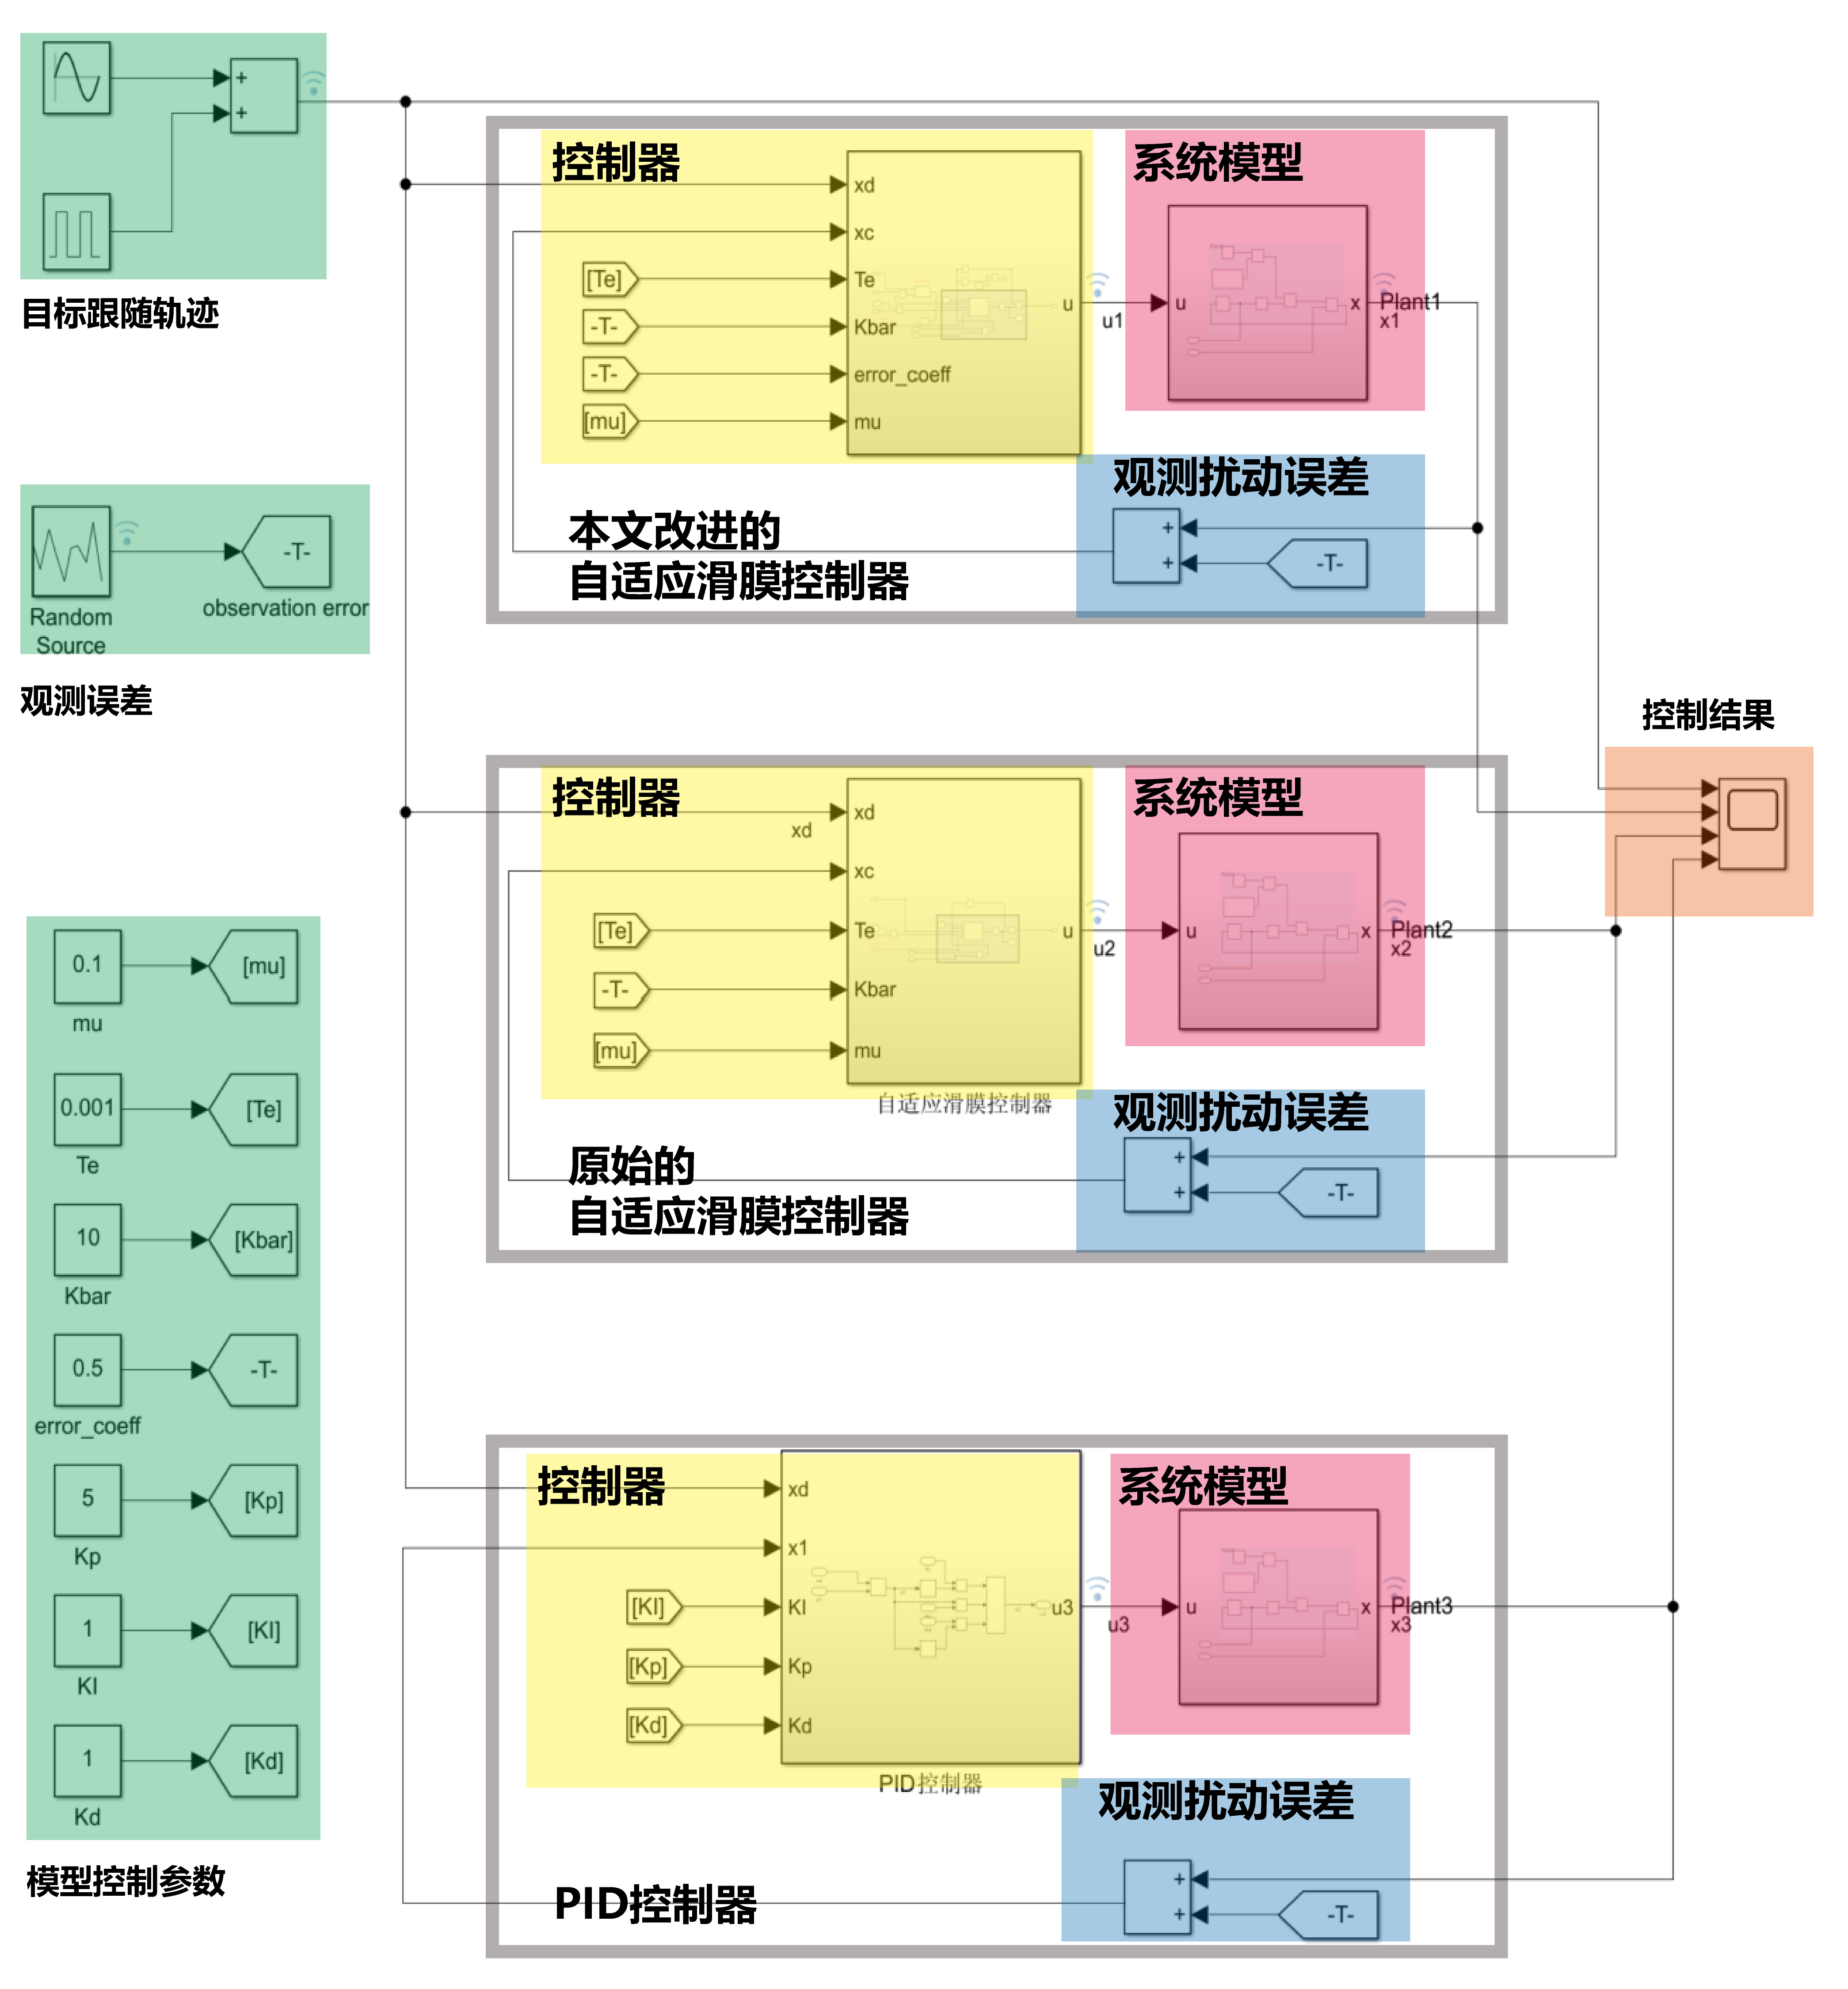
\includegraphics[width=0.6\textwidth]{imgs/simu_model.png}
    \caption{Simulink仿真模型}
    \label{fig:simu_model}
\end{figure}

整体仿真有3个控制器,分别是前文提出的改进的自适应滑膜控制器、Plestan提出的的自适应滑膜控制器和PID控制器。每个控制器接收生成的目标轨迹,做出控制响应后输出给由式子(\ref{eqn:simu_model})描述的系统模型,之后通过一个带扰动的观测器直接反馈给控制器,其中扰动误差设计为在$[0,0.05]$上均匀分布。
\FloatBarrier
\subsection{不带冲击序列的轨迹控制}

期望轨迹形式如式子(\ref{eqn:simu_xd}),其中冲击序列项系数$k_2=0$。此时三个控制器控制结果如图\ref{fig:simu_sine_trajectory}所示(其中PID控制器不收敛,故不做展示)。

\begin{figure}[H]
    \centering
    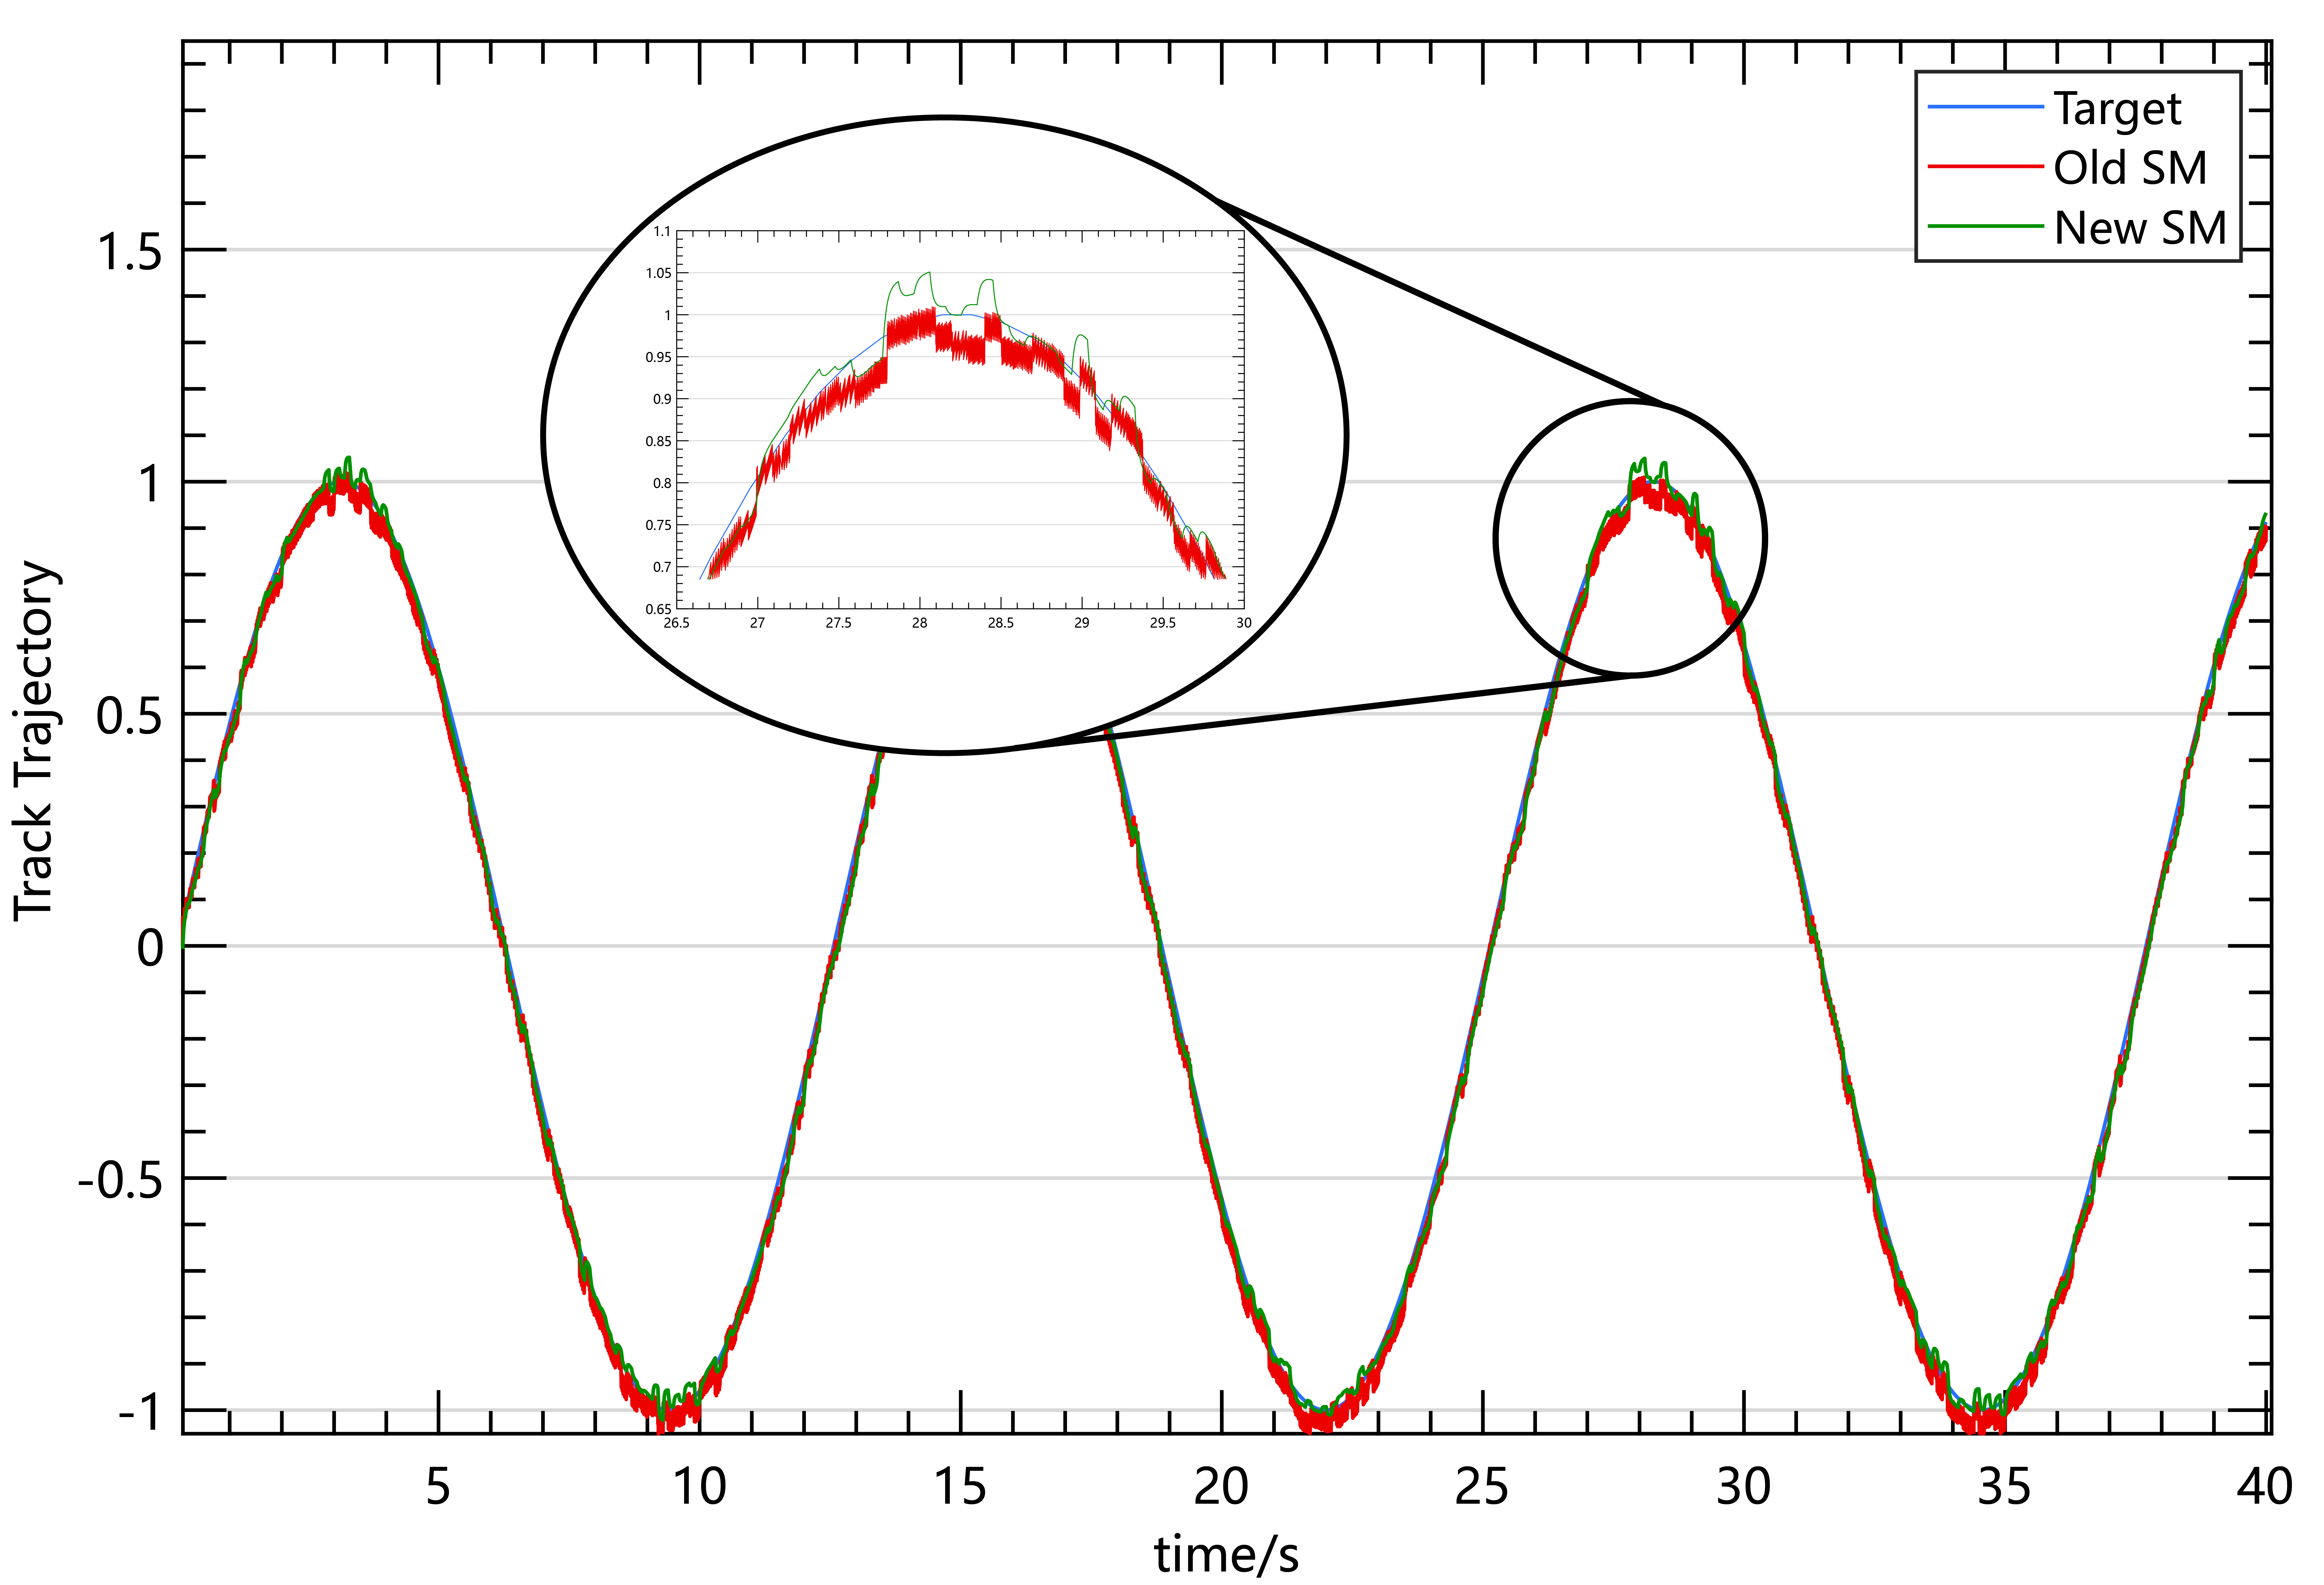
\includegraphics[width=0.6\textwidth]{imgs/simu_sine_track.png}
    \caption{自适应滑膜控制器和本文滑膜控制器的跟踪轨迹}
    \label{fig:simu_sine_trajectory}
\end{figure}

对应的跟踪误差为图\ref{fig:simu_sine_error},对应的控制器输出为图\ref{fig:simu_sine_u}。
此时,模型(\ref{eqn:simu_model})中的$a$和图\ref{fig:simu_model}中提到的观测误差$\delta$的变化如图\ref{fig:simu_model_params}所示。

\begin{figure}[H]
    \centering
    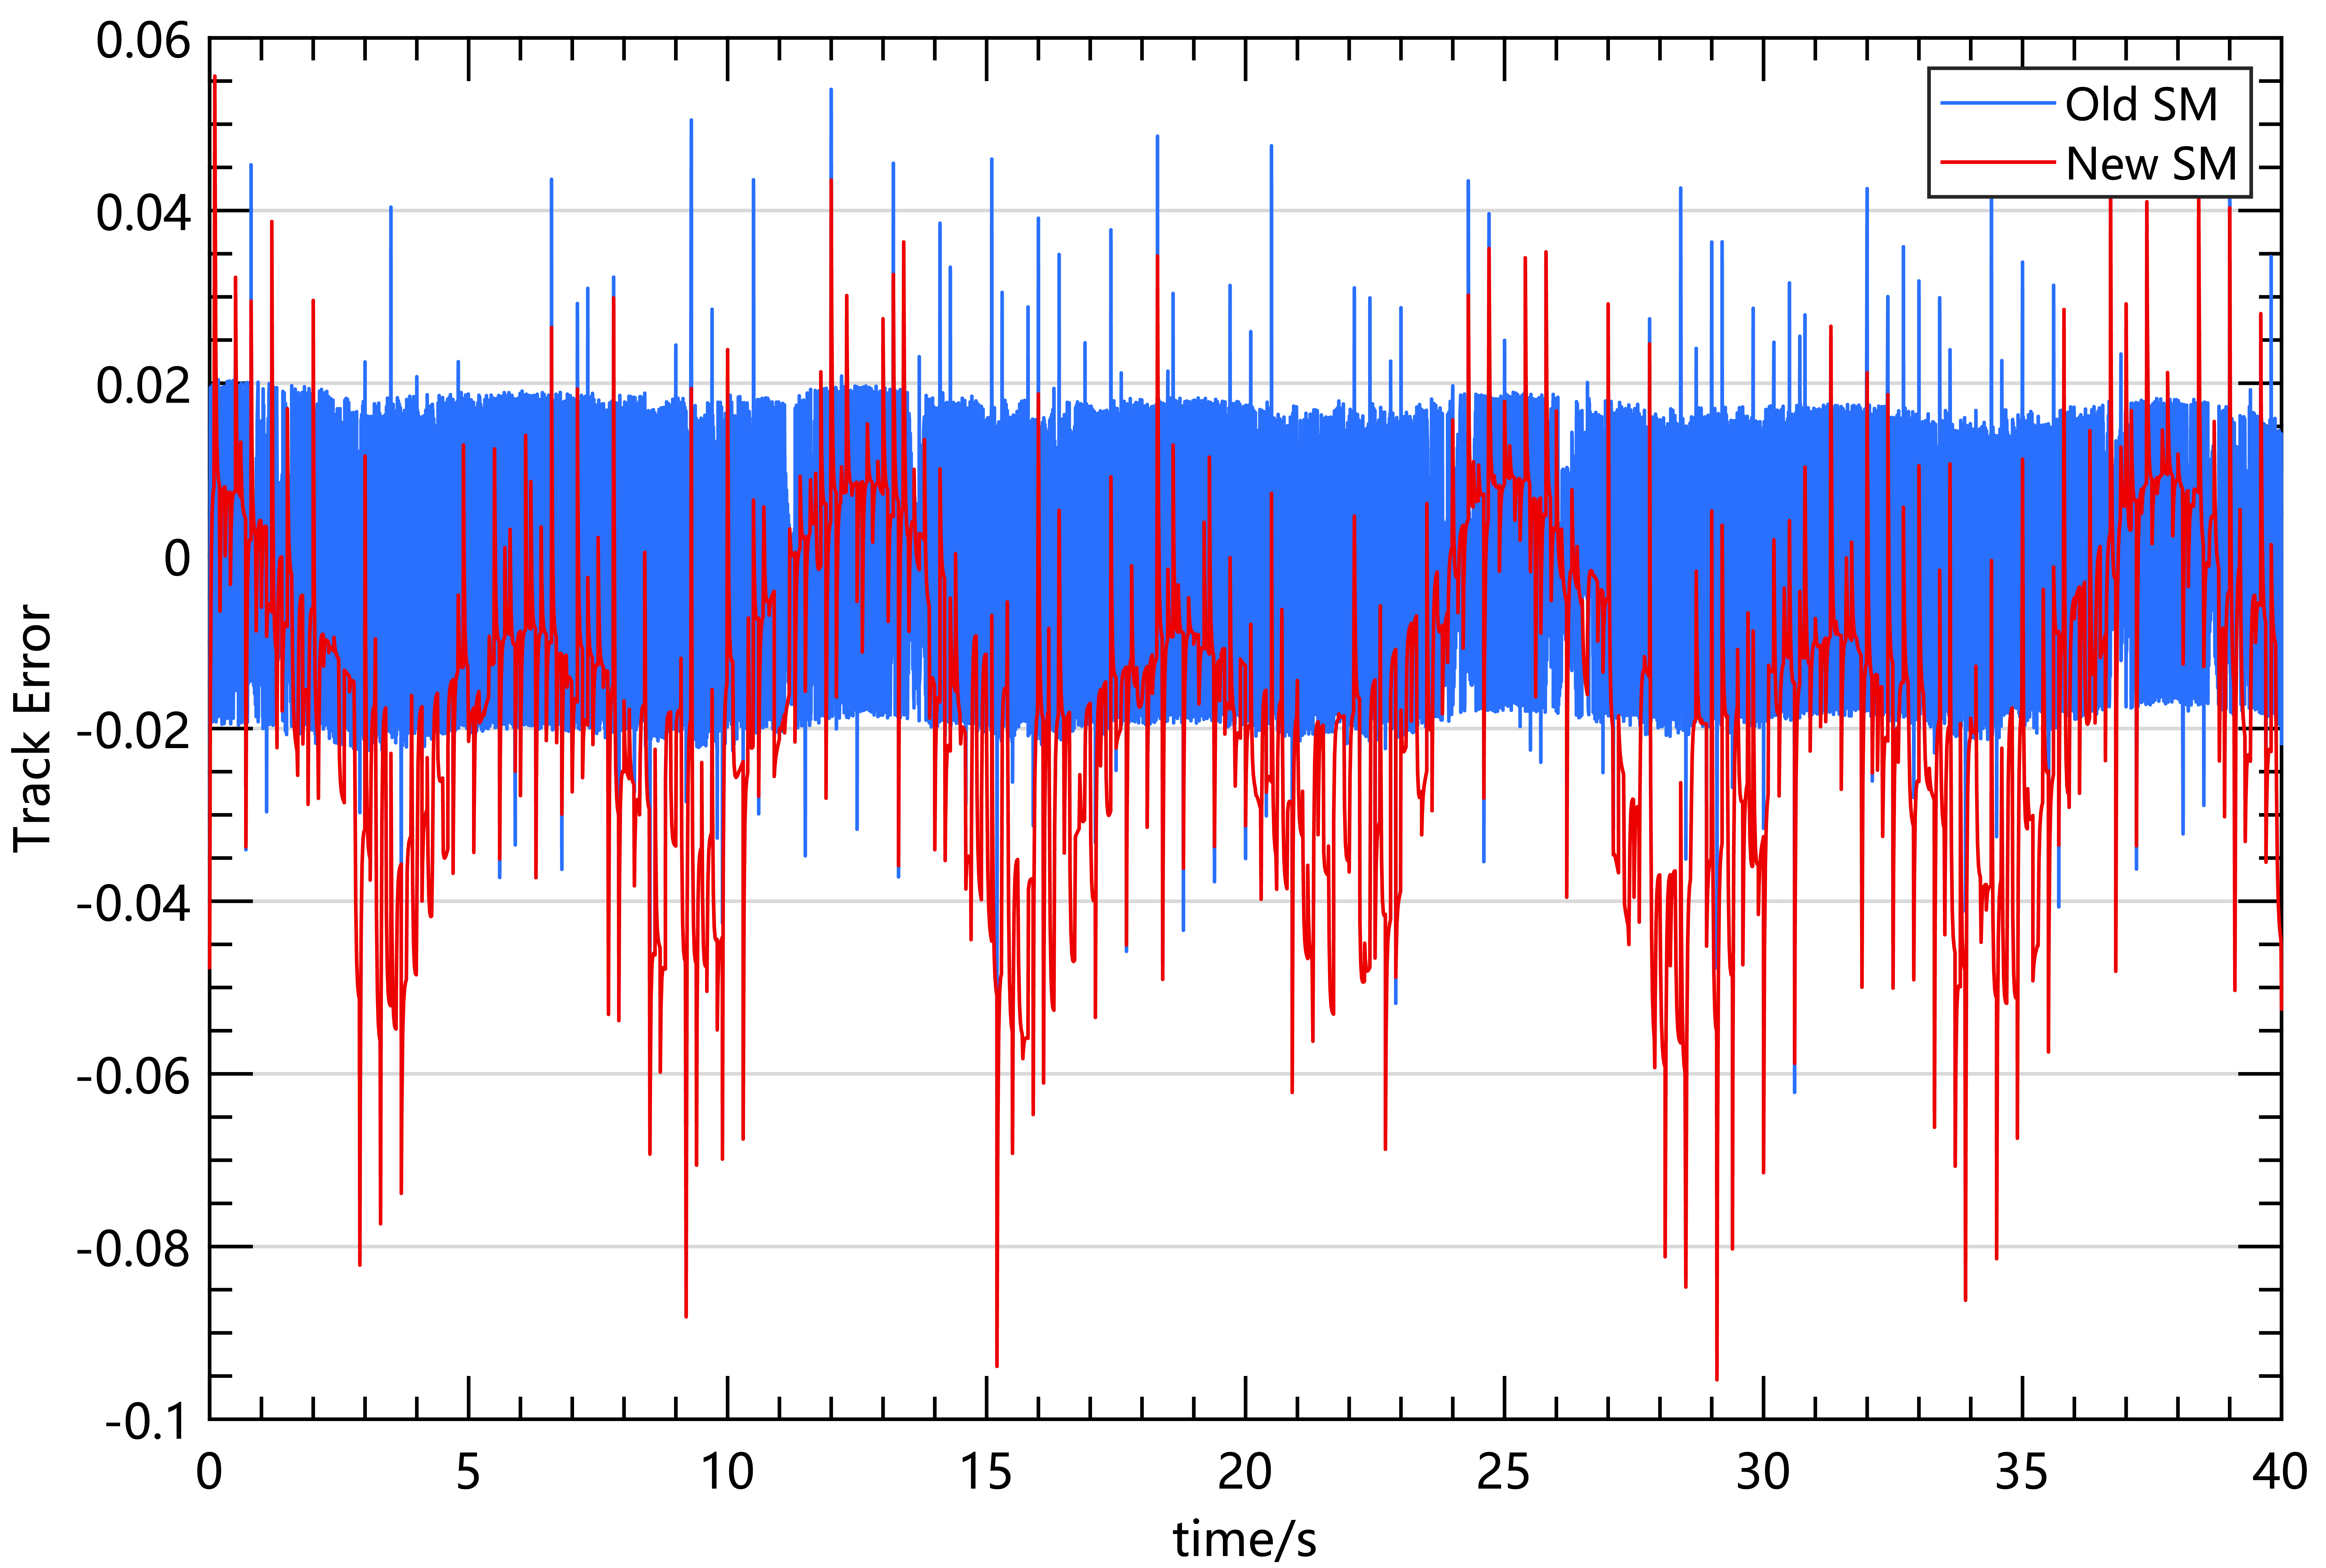
\includegraphics[width=0.6\textwidth]{imgs/simu_sine_error.png}
    \caption{自适应滑膜控制器和本文滑膜控制器的跟踪误差}
    \label{fig:simu_sine_error}
\end{figure}

\begin{figure}[H]
    \centering
    \subfloat[自适应滑膜控制器]{
    \begin{minipage}[t]{0.4\linewidth}
    \centering
    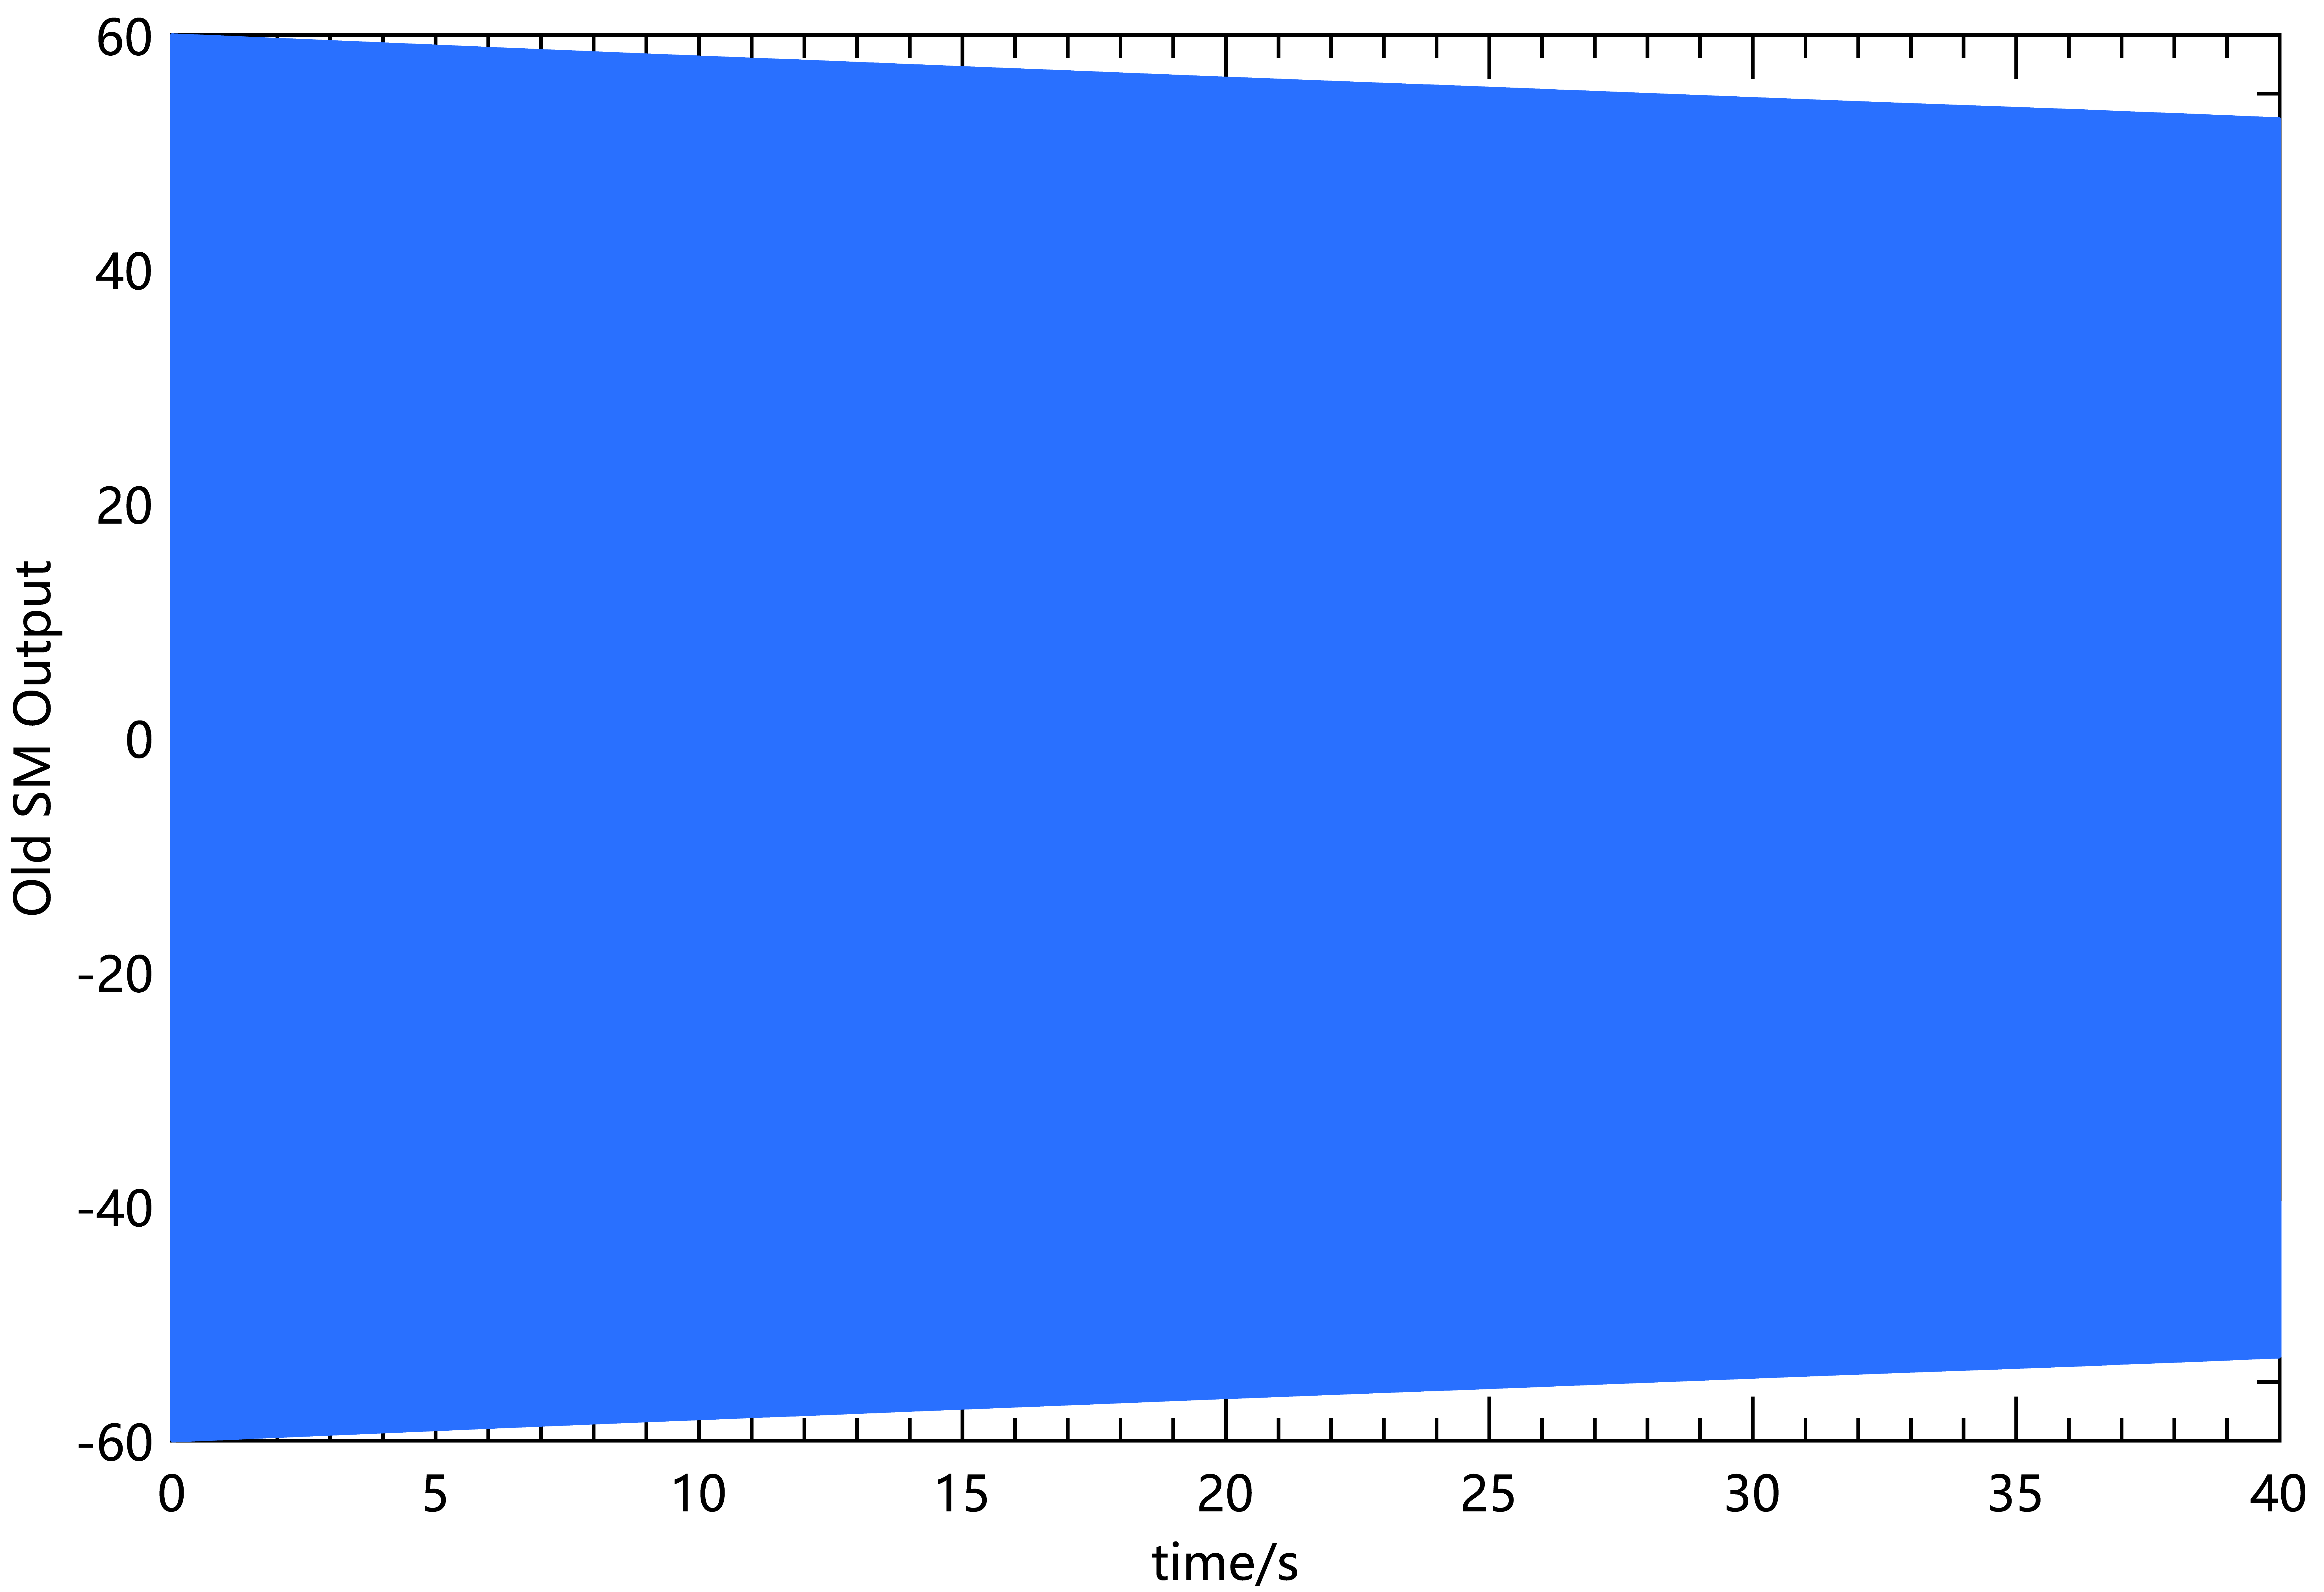
\includegraphics[width=0.9\textwidth]{imgs/simu_sine_u2.png}
    % \caption{}
    \end{minipage}%
    }%
    \hspace{0.5pt}
    \subfloat[本文自适应滑膜控制器]{
    \begin{minipage}[t]{0.4\linewidth}
    \centering
    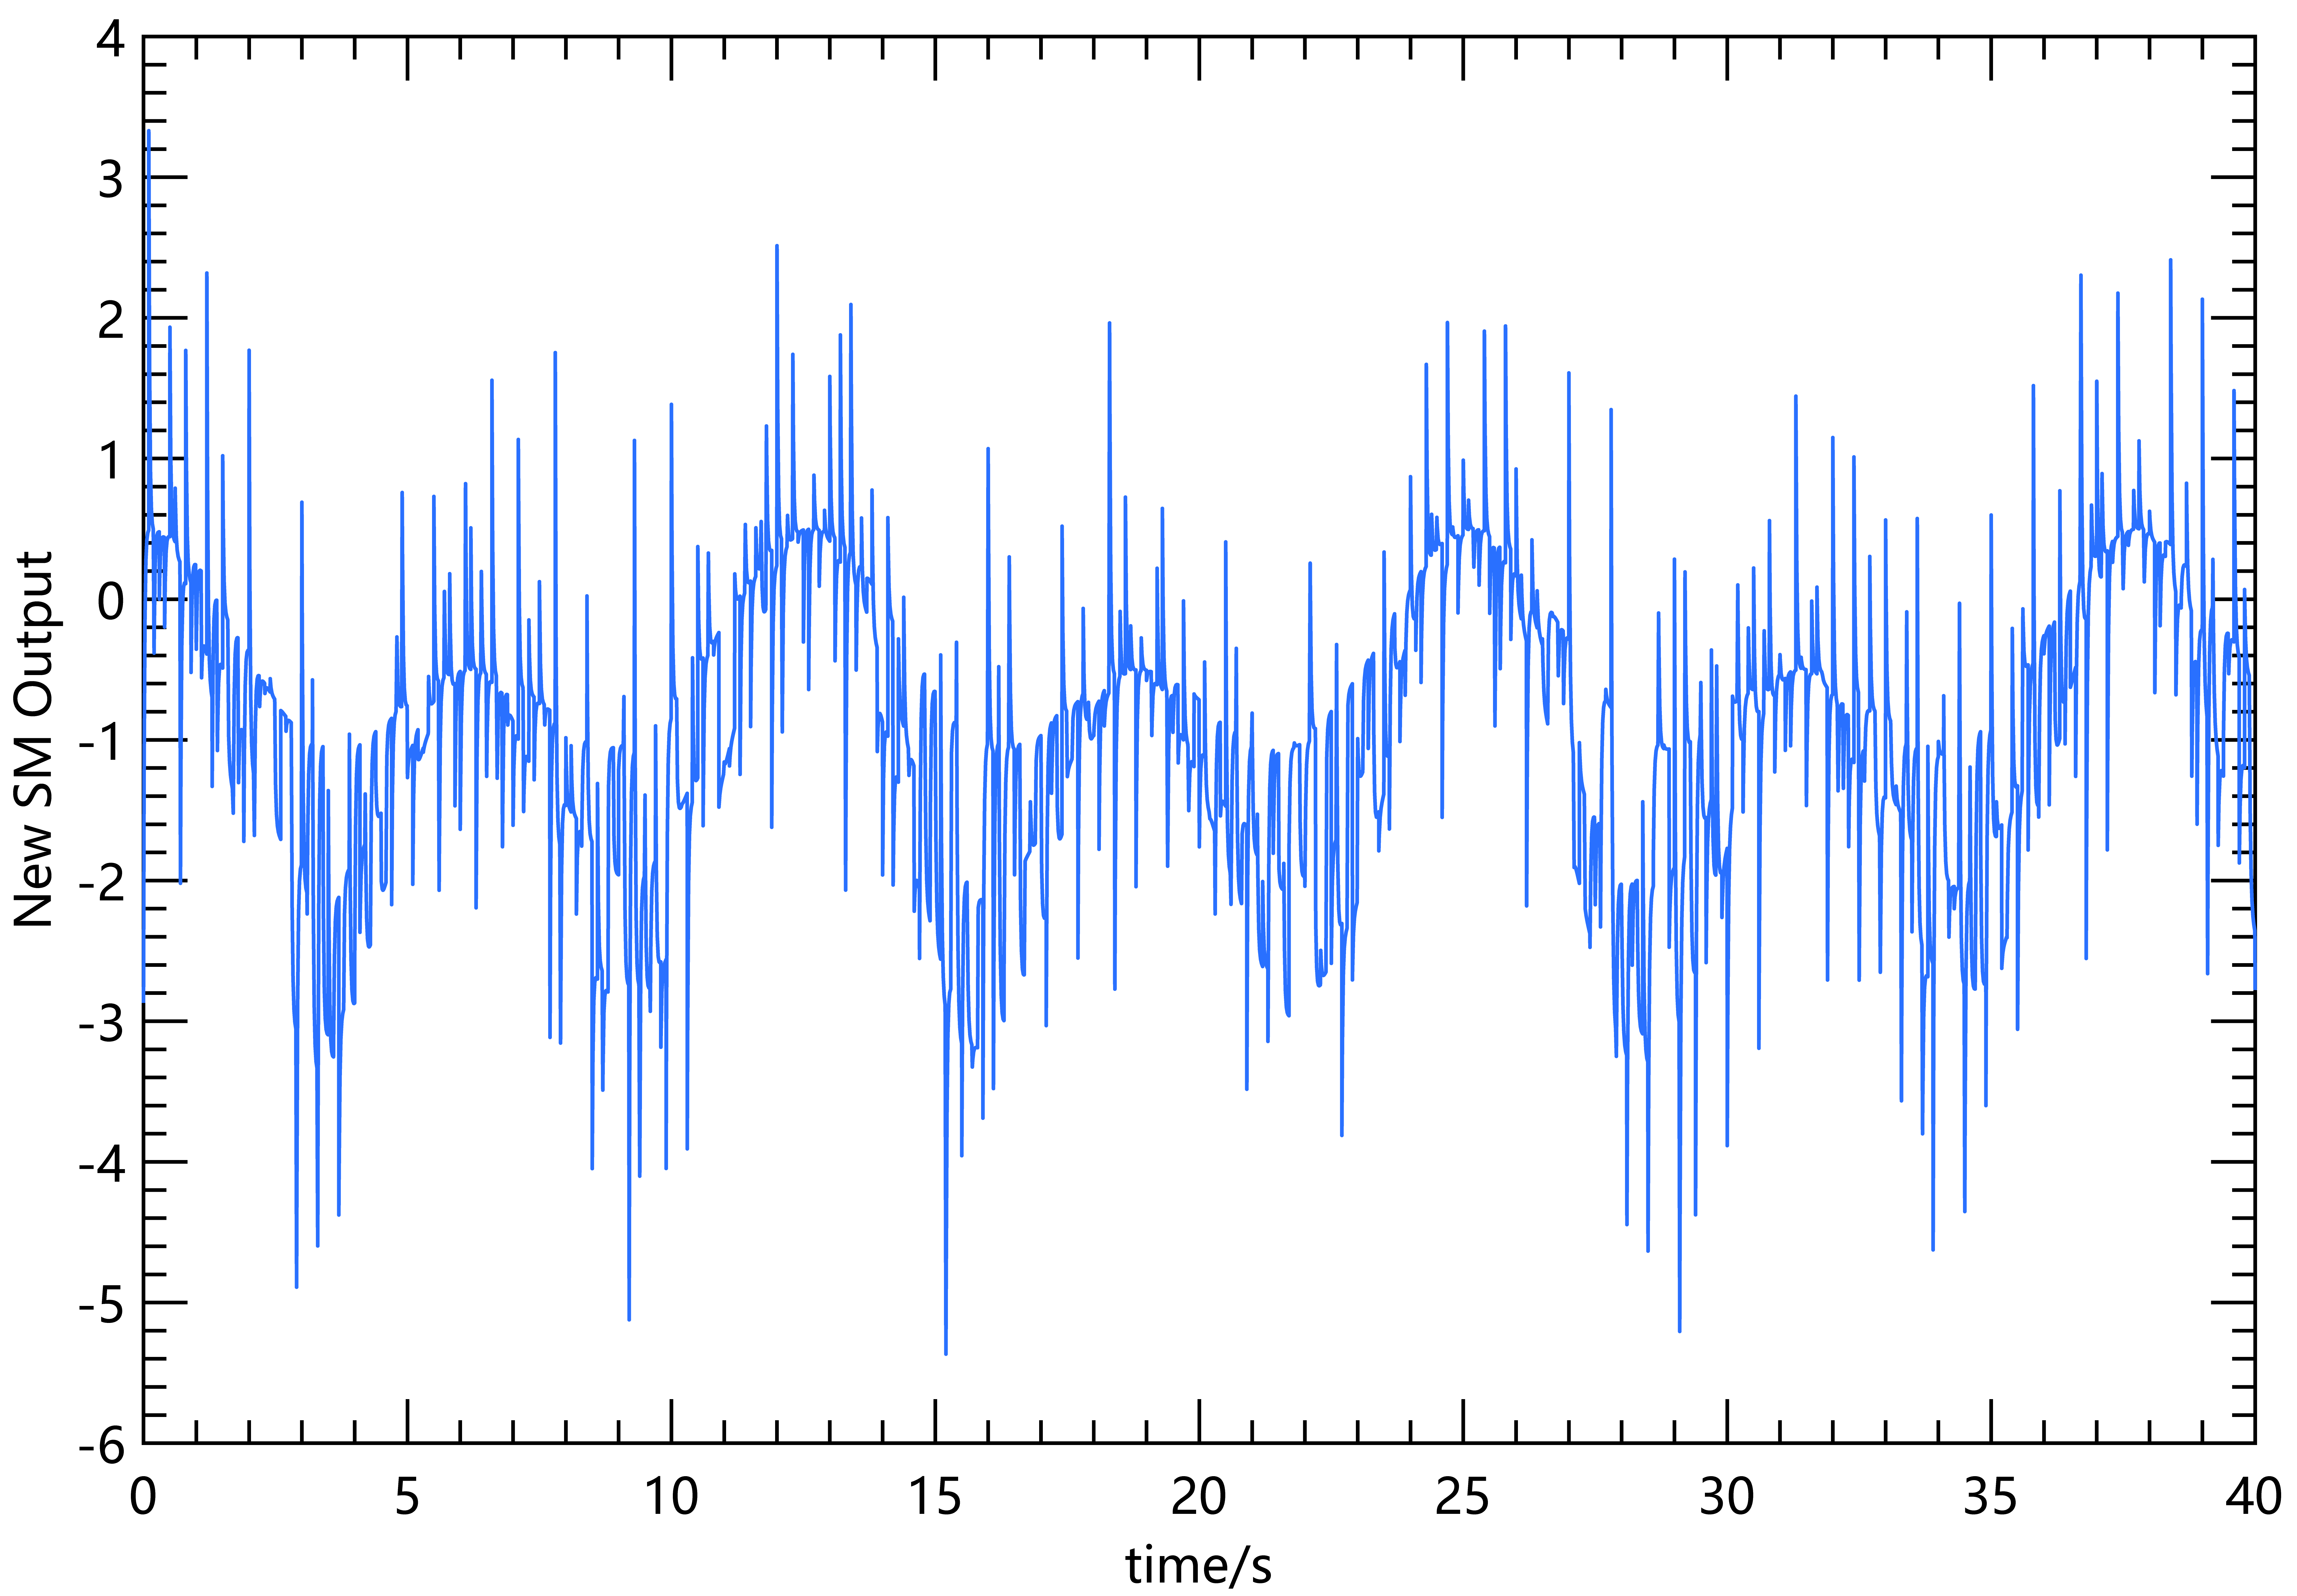
\includegraphics[width=0.9\textwidth]{imgs/simu_sine_u1.png}
    % \caption{}
    \end{minipage}%
    }%
    \centering
    \caption[]{控制器输出对比}
    \label{fig:simu_sine_u}
\end{figure}


\begin{figure}[H]
    \centering
    \subfloat[系统模型系数$a$]{
    \begin{minipage}[t]{0.4\linewidth}
    \centering
    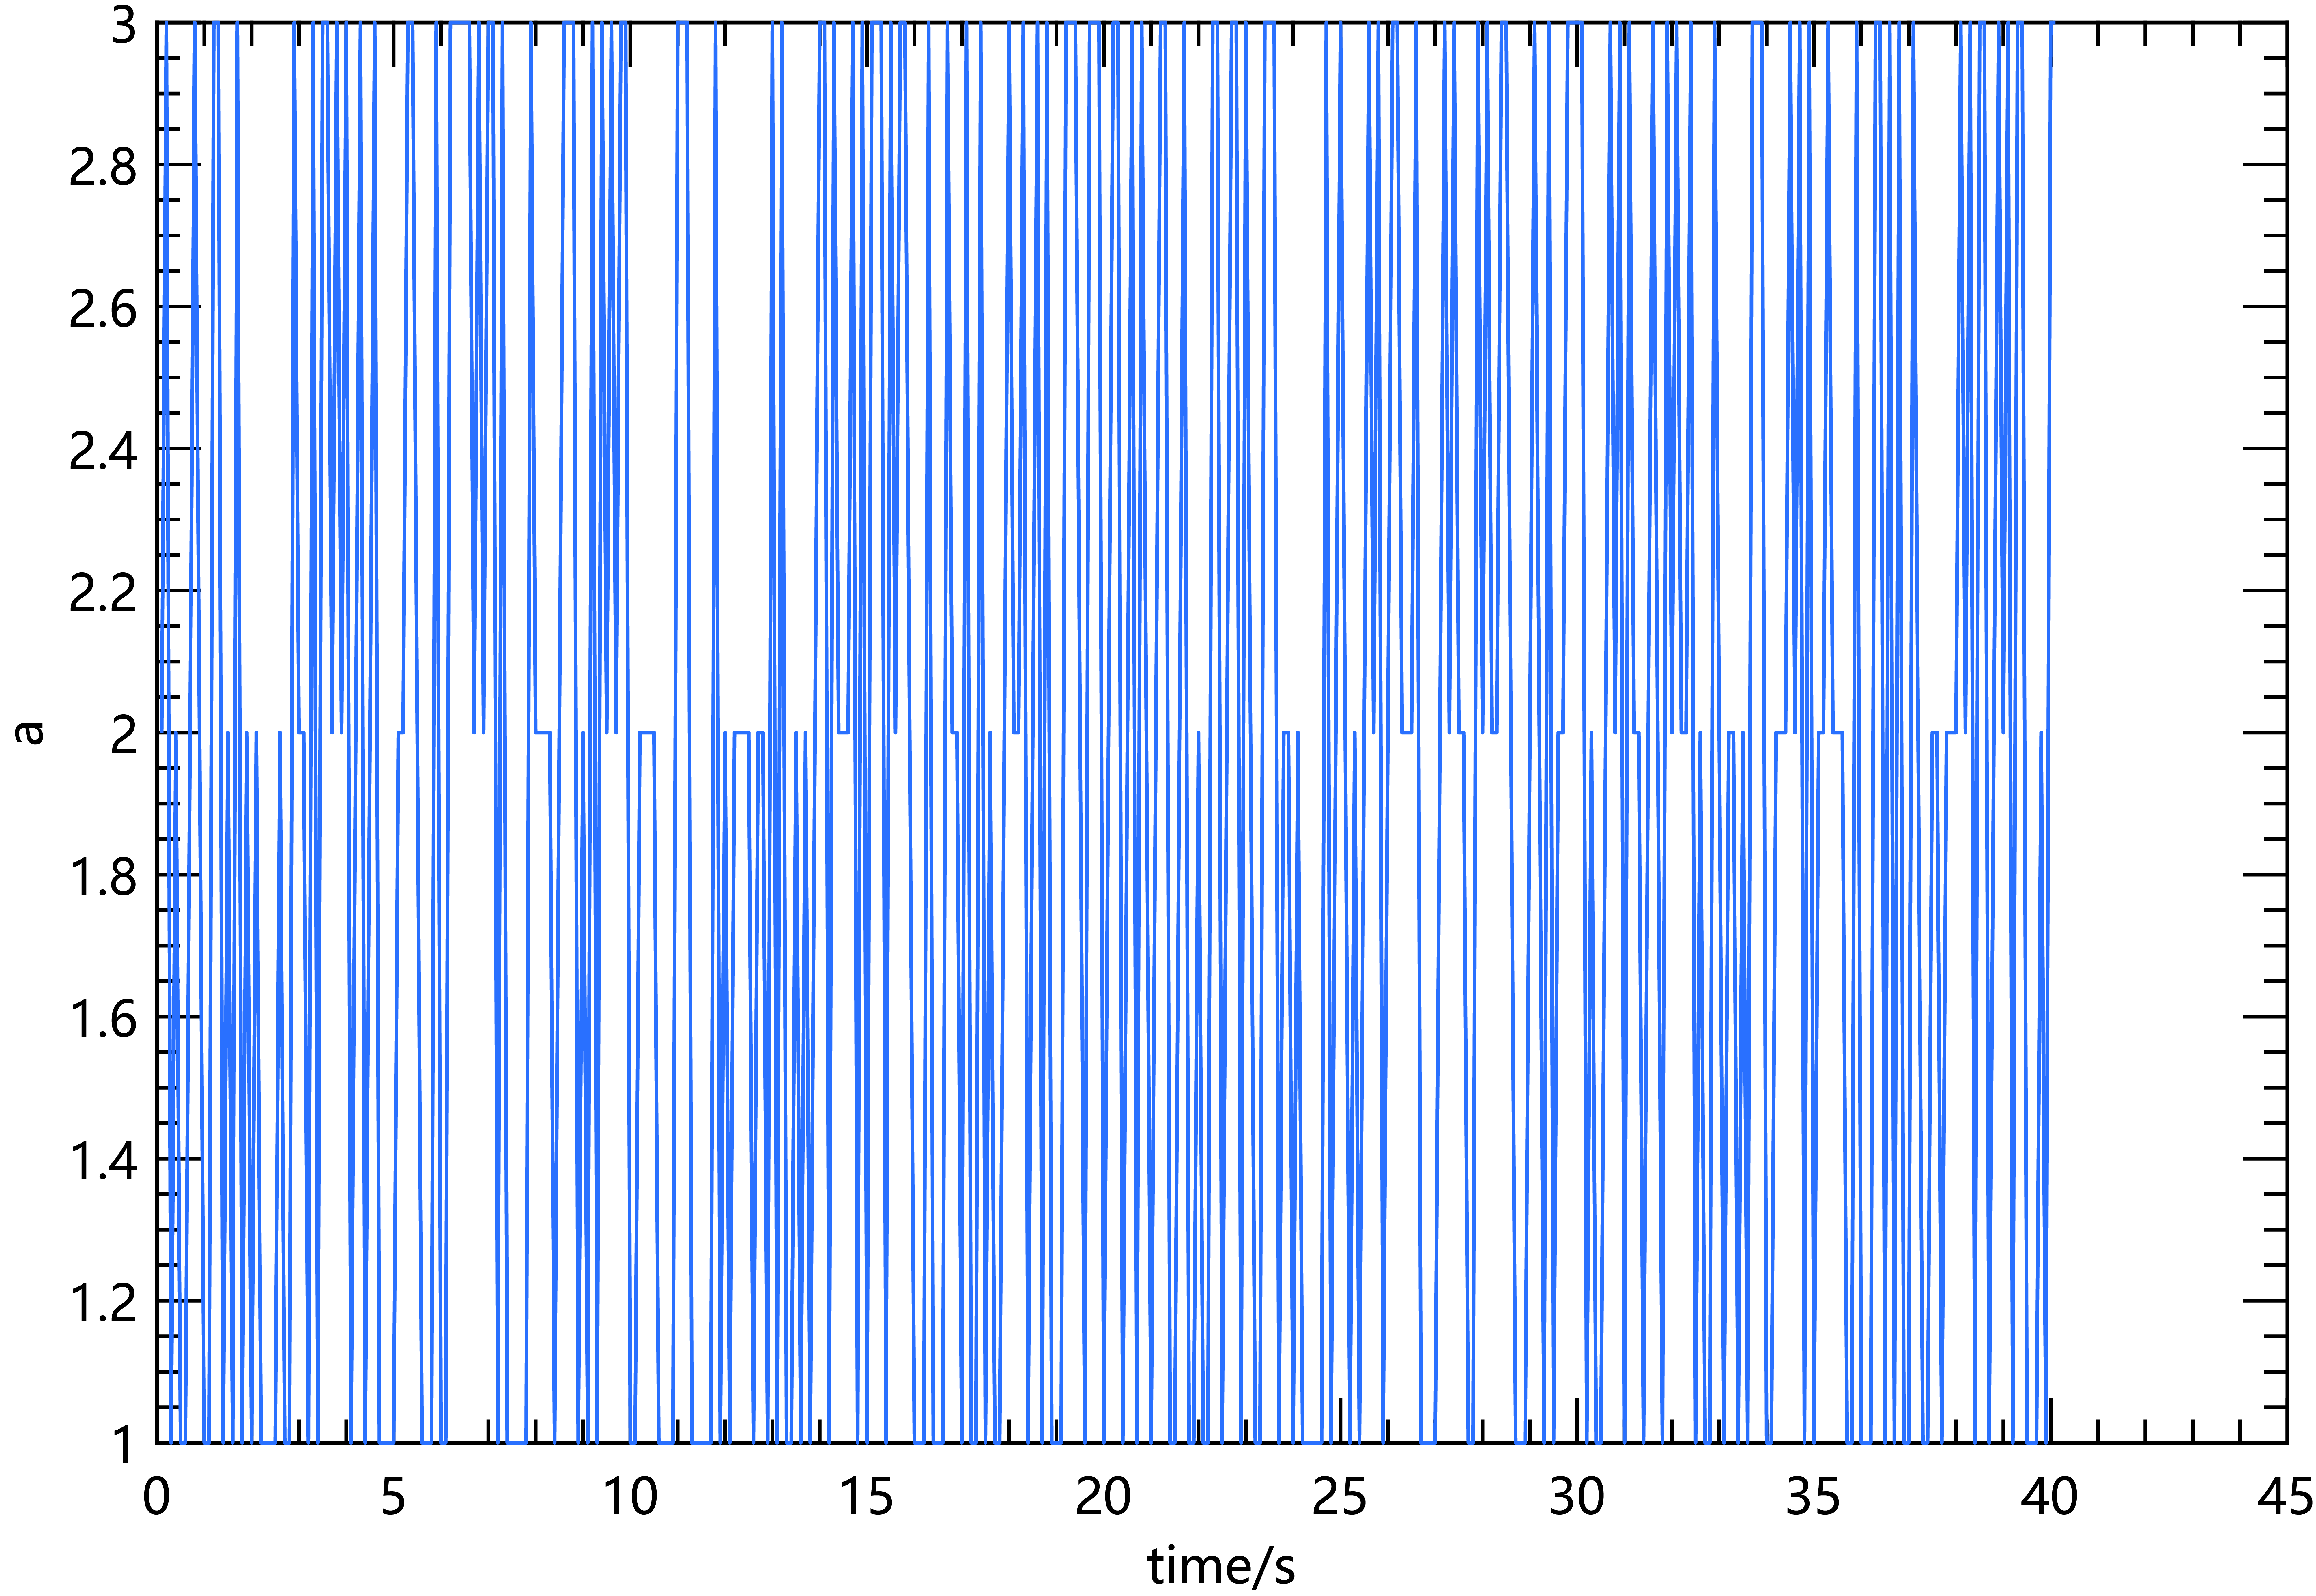
\includegraphics[width=0.9\textwidth]{imgs/simu_sine_a.png}
    % \caption{}
    \end{minipage}%
    }%
    \hspace{0.5pt}
    \subfloat[模型观测误差$\delta$]{
    \begin{minipage}[t]{0.4\linewidth}
    \centering
    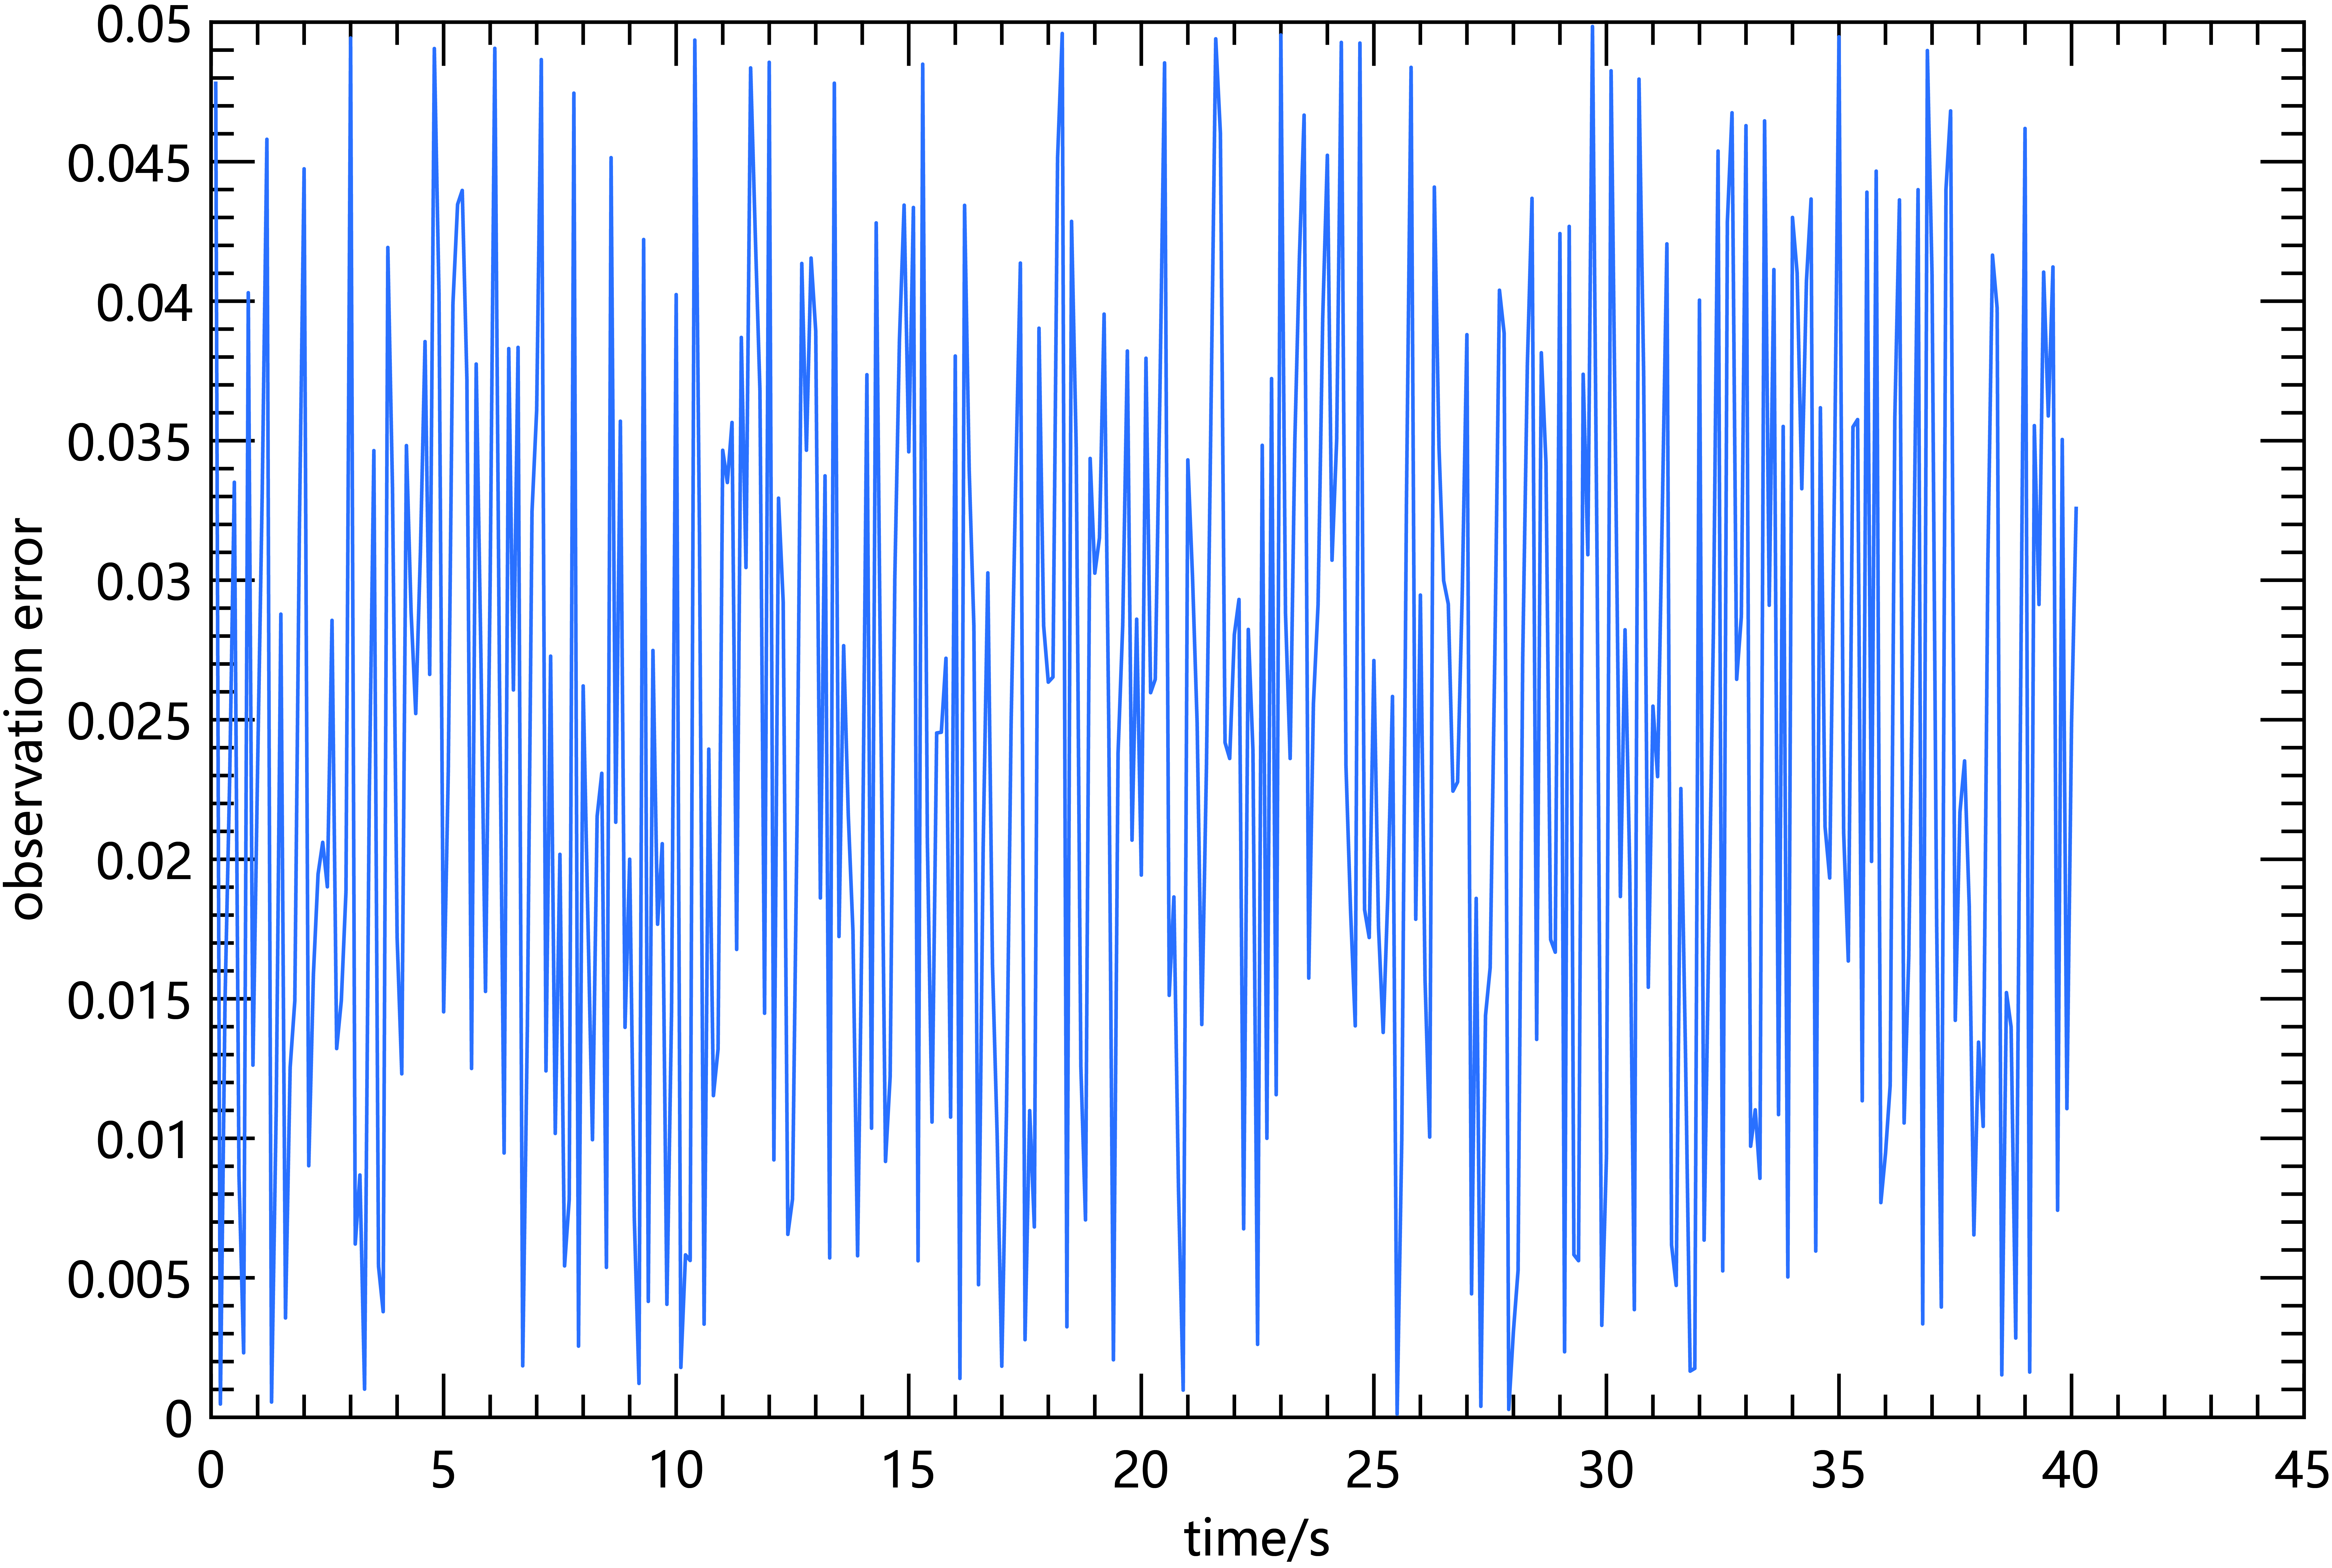
\includegraphics[width=0.9\textwidth]{imgs/simu_sine_observation.png}
    % \caption{}
    \end{minipage}%
    }%
    \centering
    \caption[]{仿真模型参数变化}
    \label{fig:simu_model_params}
\end{figure}

可以发现,在观测误差$\delta$在$[0, 0.05]$之间均匀变化、系统模型参数$a$在$\{1,2,3\}$之间随机变化的情况下,
除了PID控制器之外的两个自适应滑膜控制器都能够做到比较好的跟踪效果,其中自适应控制器的控制误差主要分布在
$\left[ -0.02,0.02 \right] $之间,本文提出的控制器控制误差主要分布在$\left[ -0.06,0.01 \right] $之间,但本文控制器输出的跟踪位移明显比自适应控制器平滑,其抖动弱了很多。此外,误差在正弦曲线取极值的时候达到最大,在正弦曲线速度变化最大的中端跟踪效果比较好,这表明提出的控制器可以比较好地跟踪变化的输入。

对比两个控制器的输出,可以发现自适应滑膜控制器依赖高频变化、幅值大的控制输入,从而不断控制系统稳定在输入轨迹附近;本文提出的控制器输出则输出范围小,频率低,达到的误差控制效果虽然相对差一点,但其可以直接应用到实际的物理系统上,在后文中的实物实验上也可以发现这一优点。
\FloatBarrier
\subsection{带冲击序列的轨迹控制}

期望轨迹形式如式子(\ref{eqn:simu_xd}),其中冲击序列项系数$k_2=1$。此时三个控制器控制结果如图\ref{fig:simu_pulse_sine_trajectory}所示(其中PID控制器不收敛,故不做展示)。

\begin{figure}[H]
    \centering
    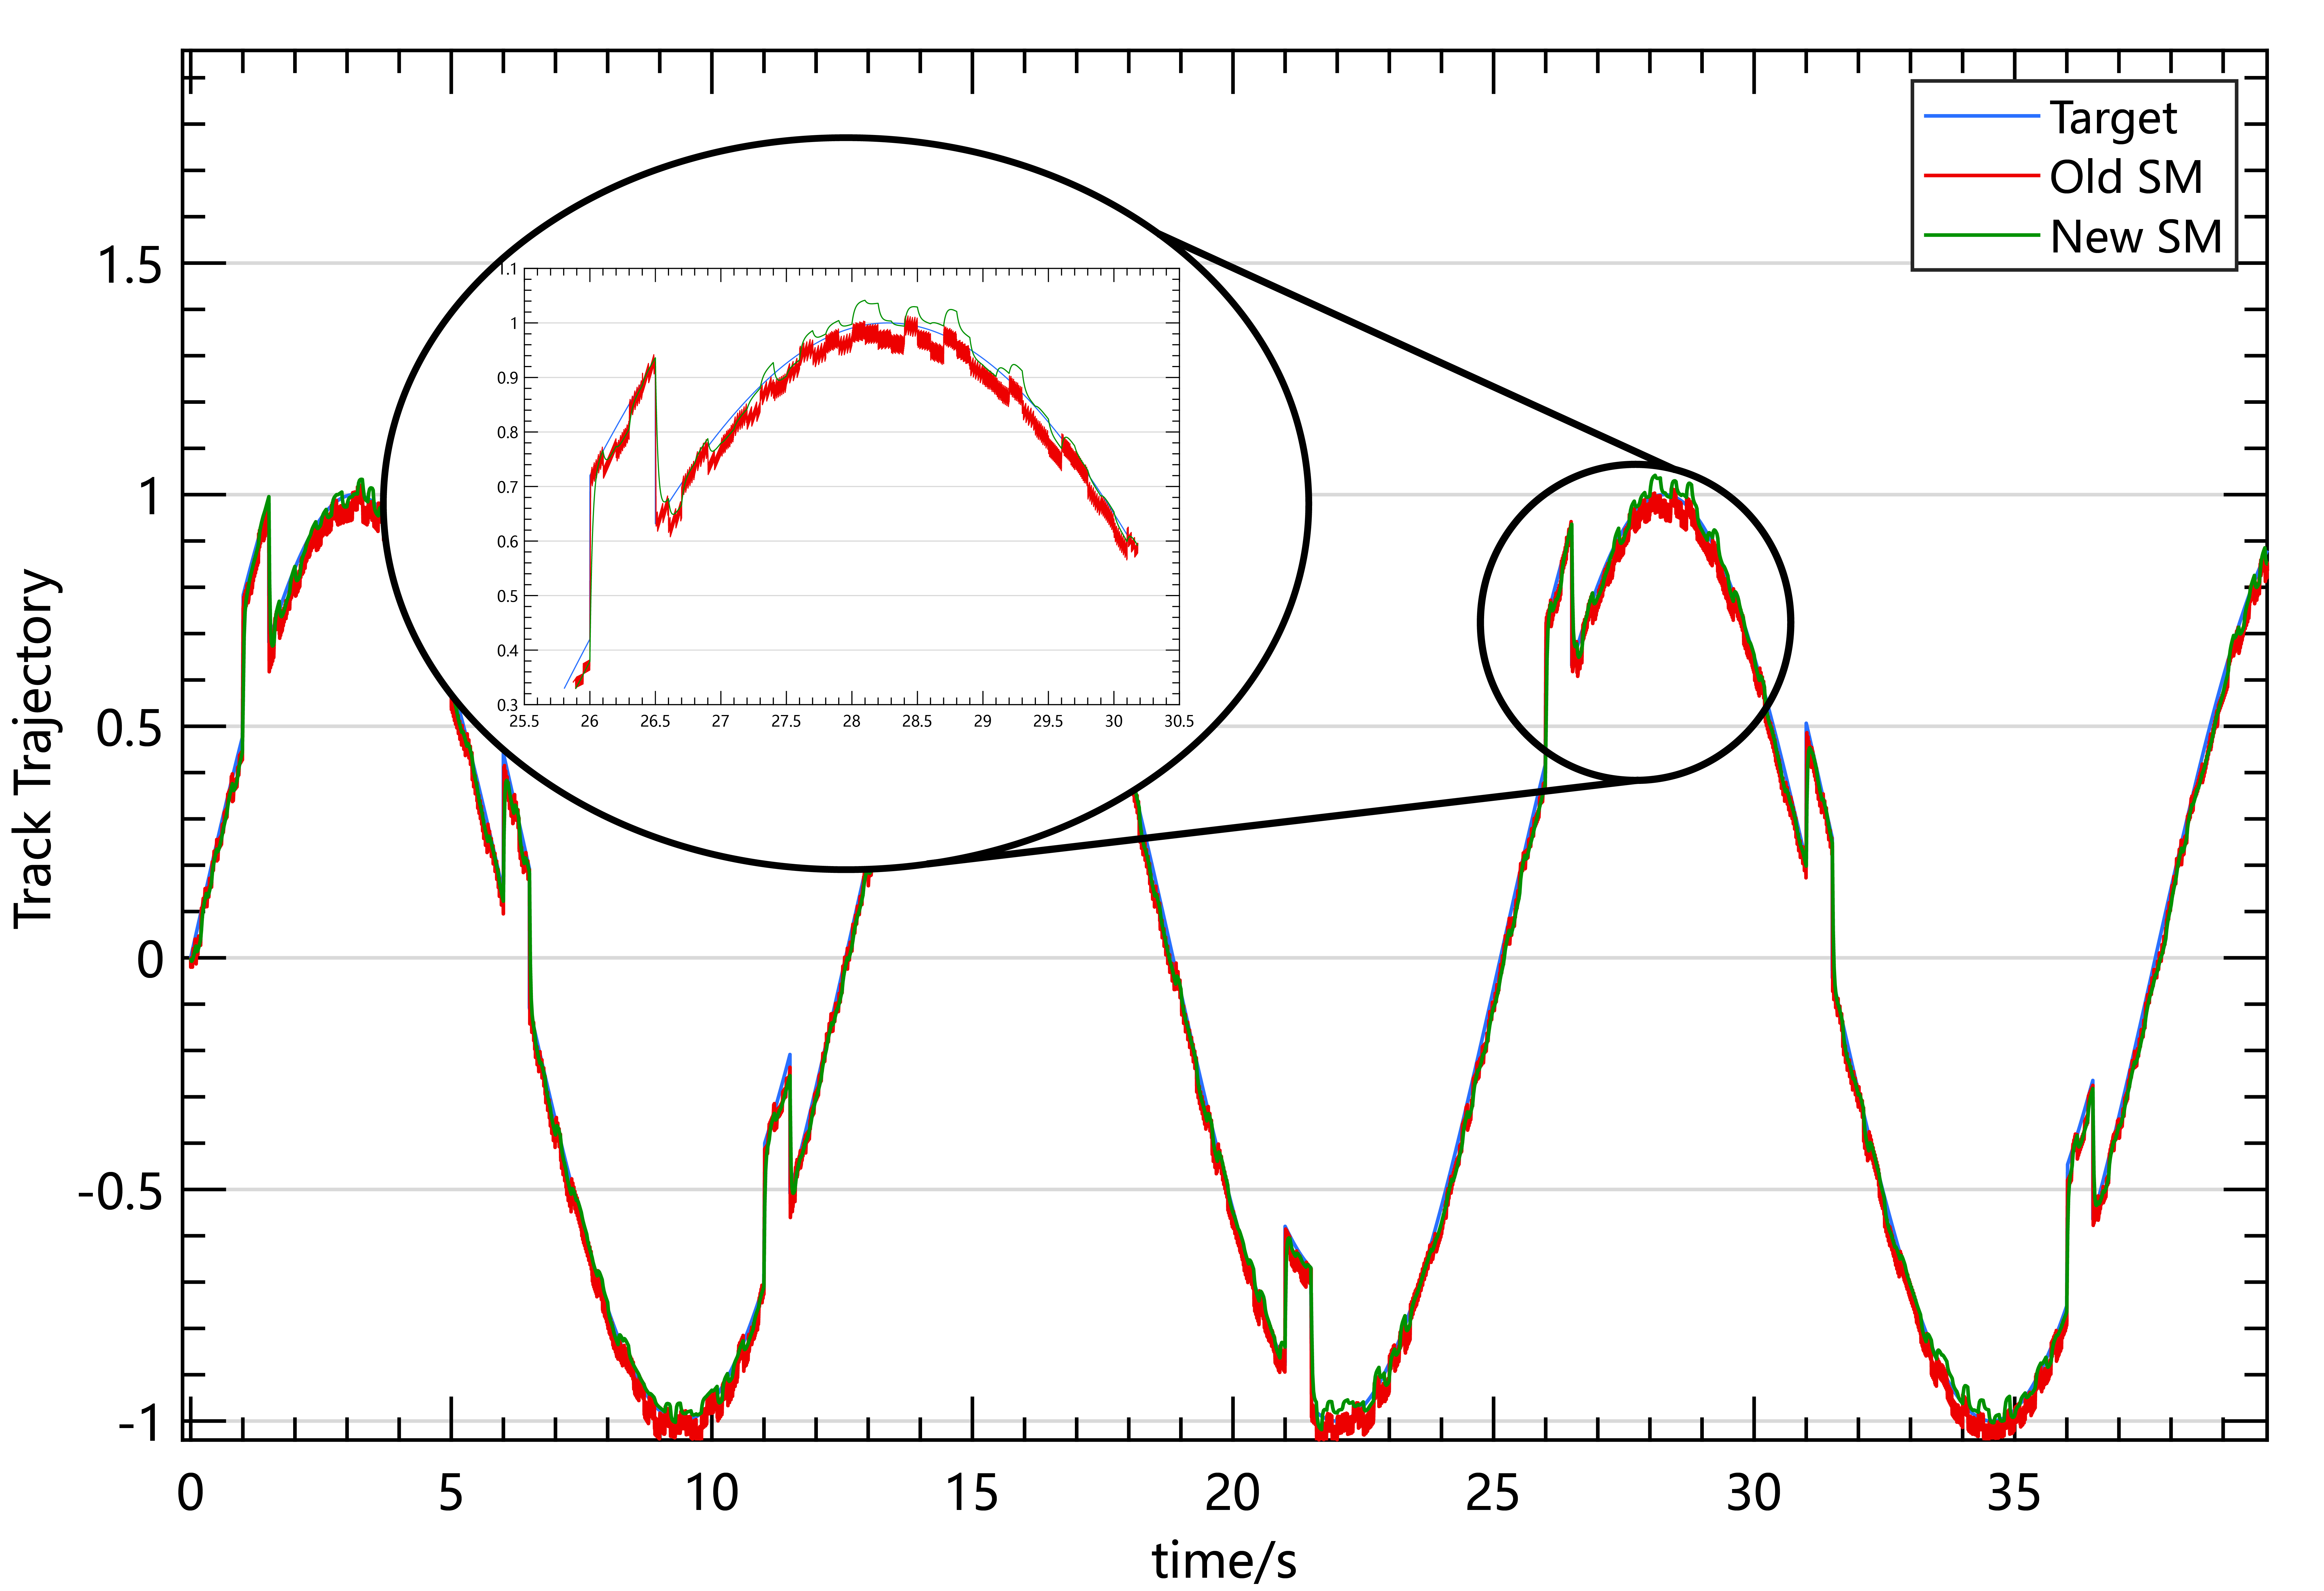
\includegraphics[width=0.6\textwidth]{imgs/simu_pulse_sine_track.png}
    \caption{自适应滑膜控制器和本文滑膜控制器的跟踪轨迹}
    \label{fig:simu_pulse_sine_trajectory}
\end{figure}

对应的跟踪误差为图\ref{fig:simu_pulse_sine_error},对应的控制器输出为图\ref{fig:simu_pulse_sine_u}。此时,模型(\ref{eqn:simu_model})中的$a$和图\ref{fig:simu_model}中提到的观测误差$\delta$的变化也满足图\ref{fig:simu_model_params}中的变化情况。

\begin{figure}[H]
    \centering
    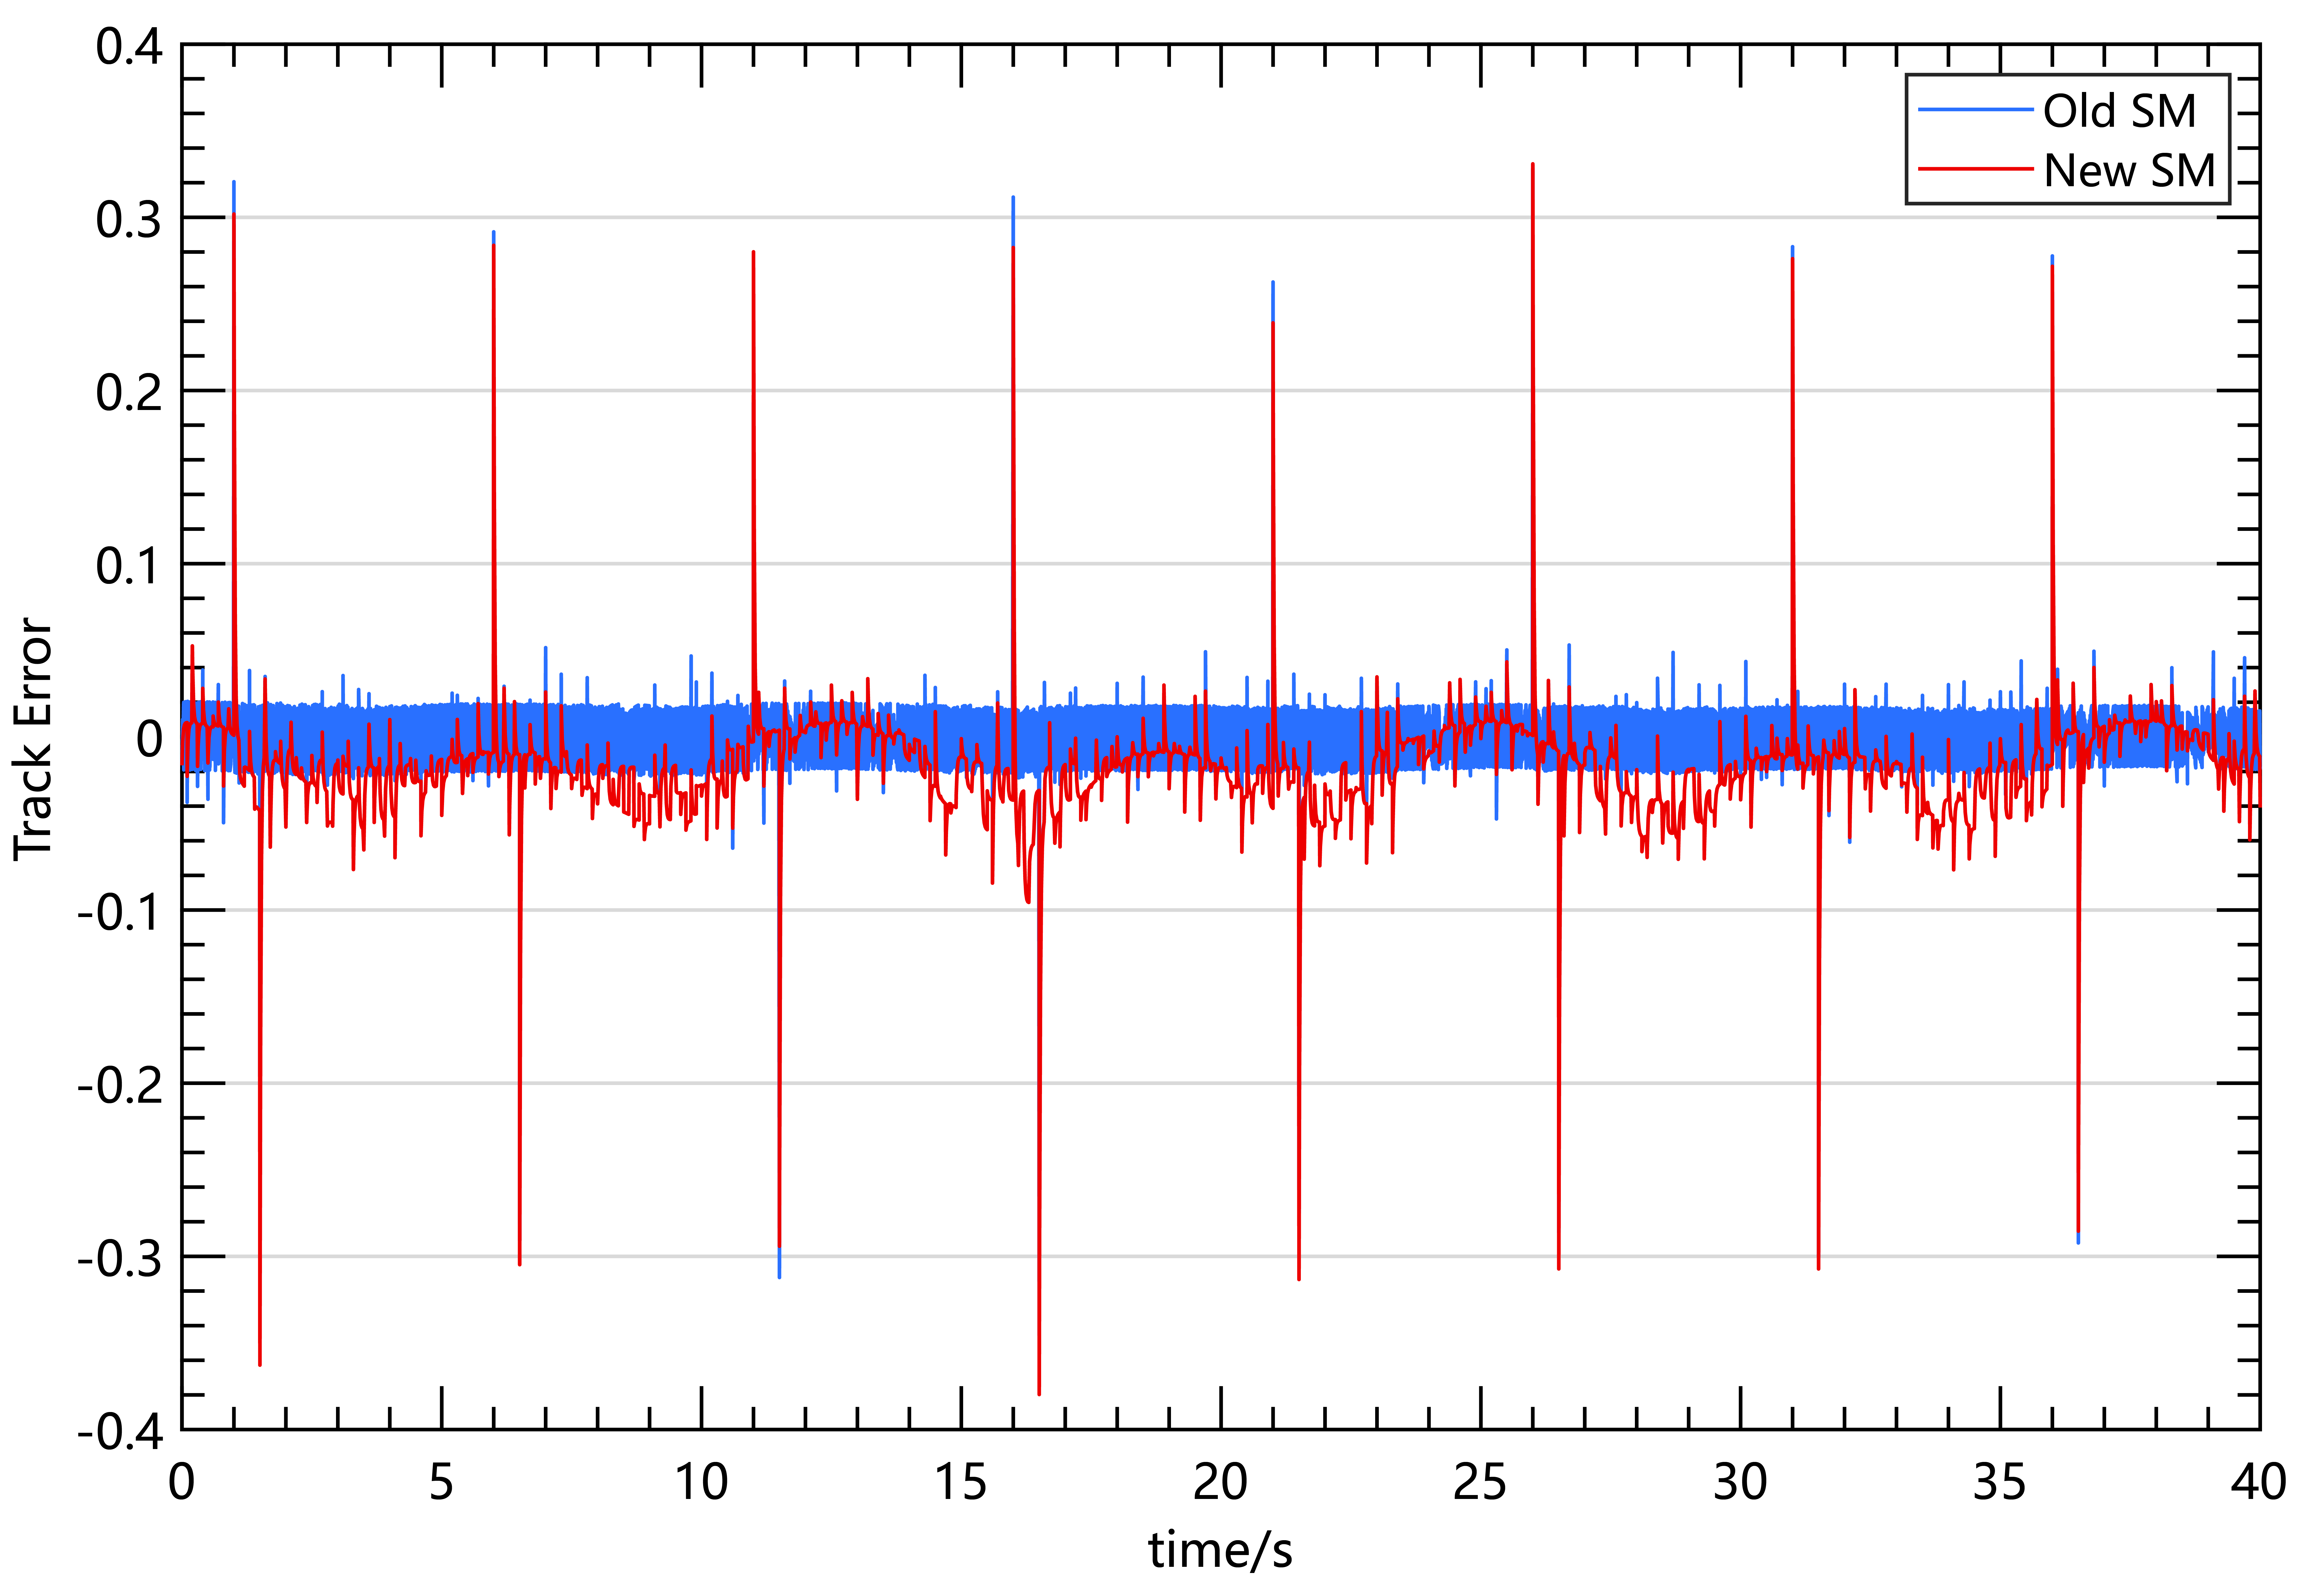
\includegraphics[width=0.6\textwidth]{imgs/simu_pulse_sine_error.png}
    \caption{自适应滑膜控制器和本文滑膜控制器的跟踪误差}
    \label{fig:simu_pulse_sine_error}
\end{figure}

\begin{figure}[H]
    \centering
    \subfloat[自适应滑膜控制器]{
    \begin{minipage}[t]{0.4\linewidth}
    \centering
    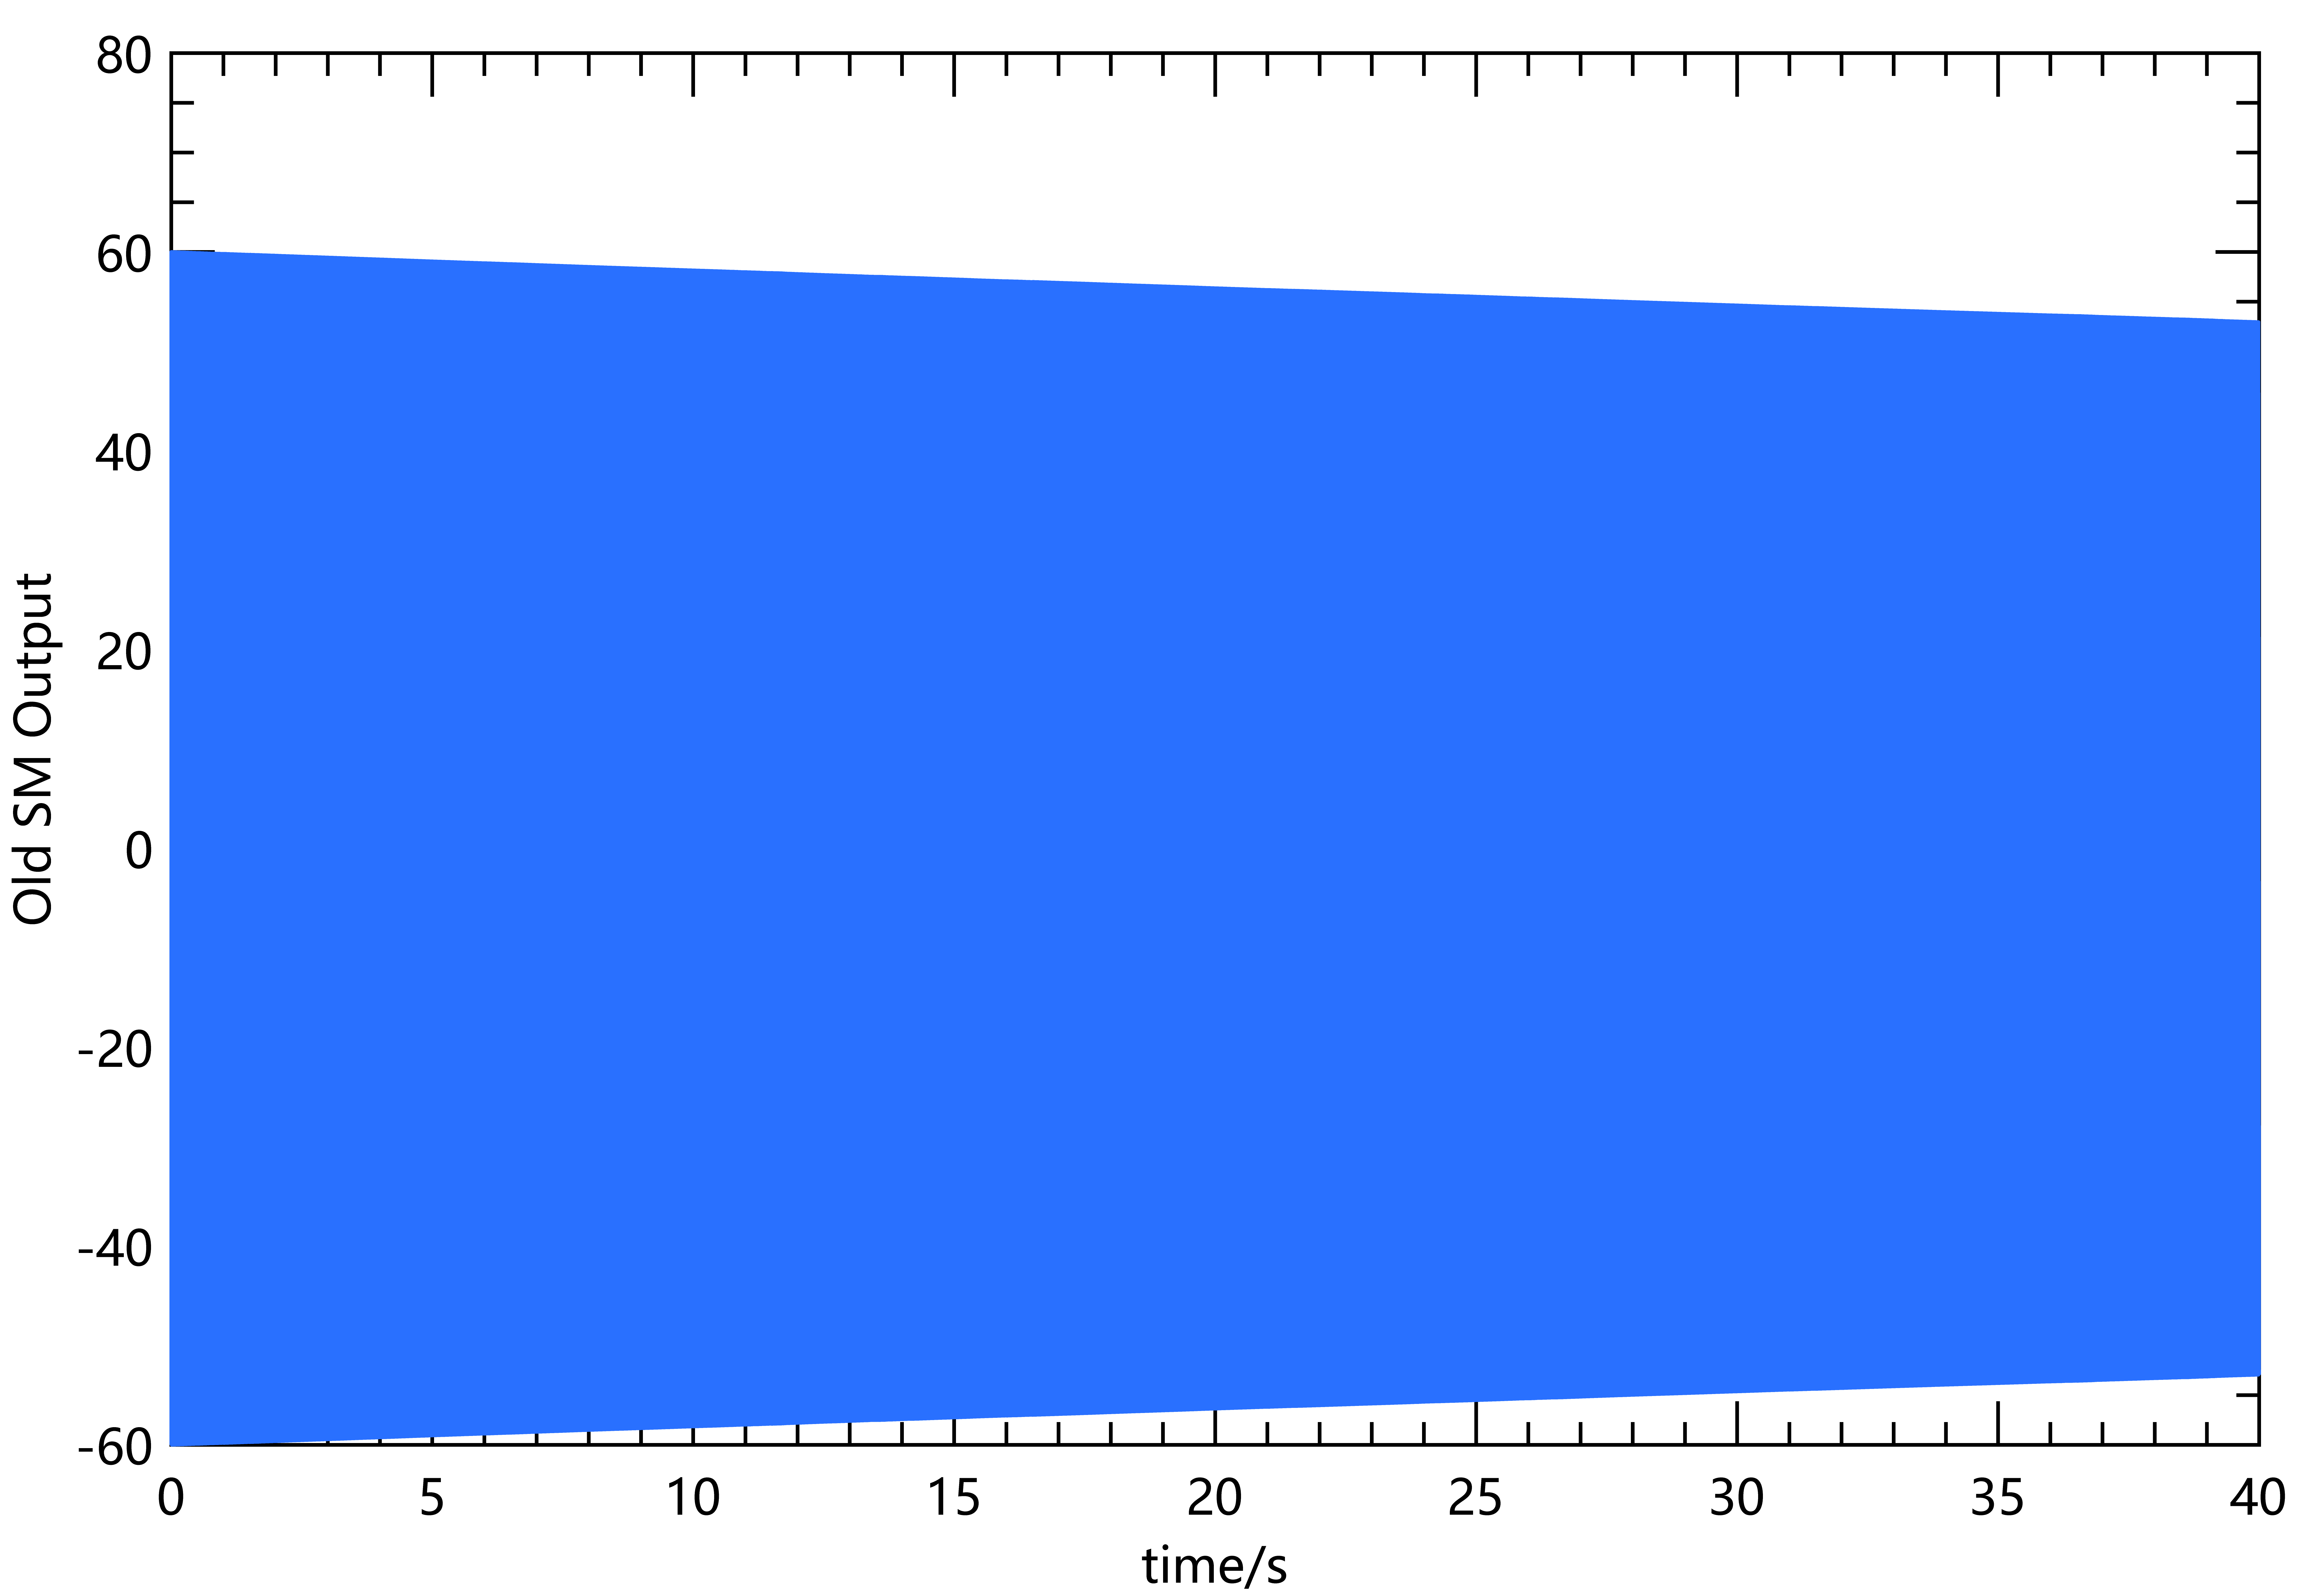
\includegraphics[width=0.9\textwidth]{imgs/simu_pulse_sine_u2.png}
    % \caption{}
    \end{minipage}%
    }%
    \hspace{0.5pt}
    \subfloat[本文自适应滑膜控制器]{
    \begin{minipage}[t]{0.4\linewidth}
    \centering
    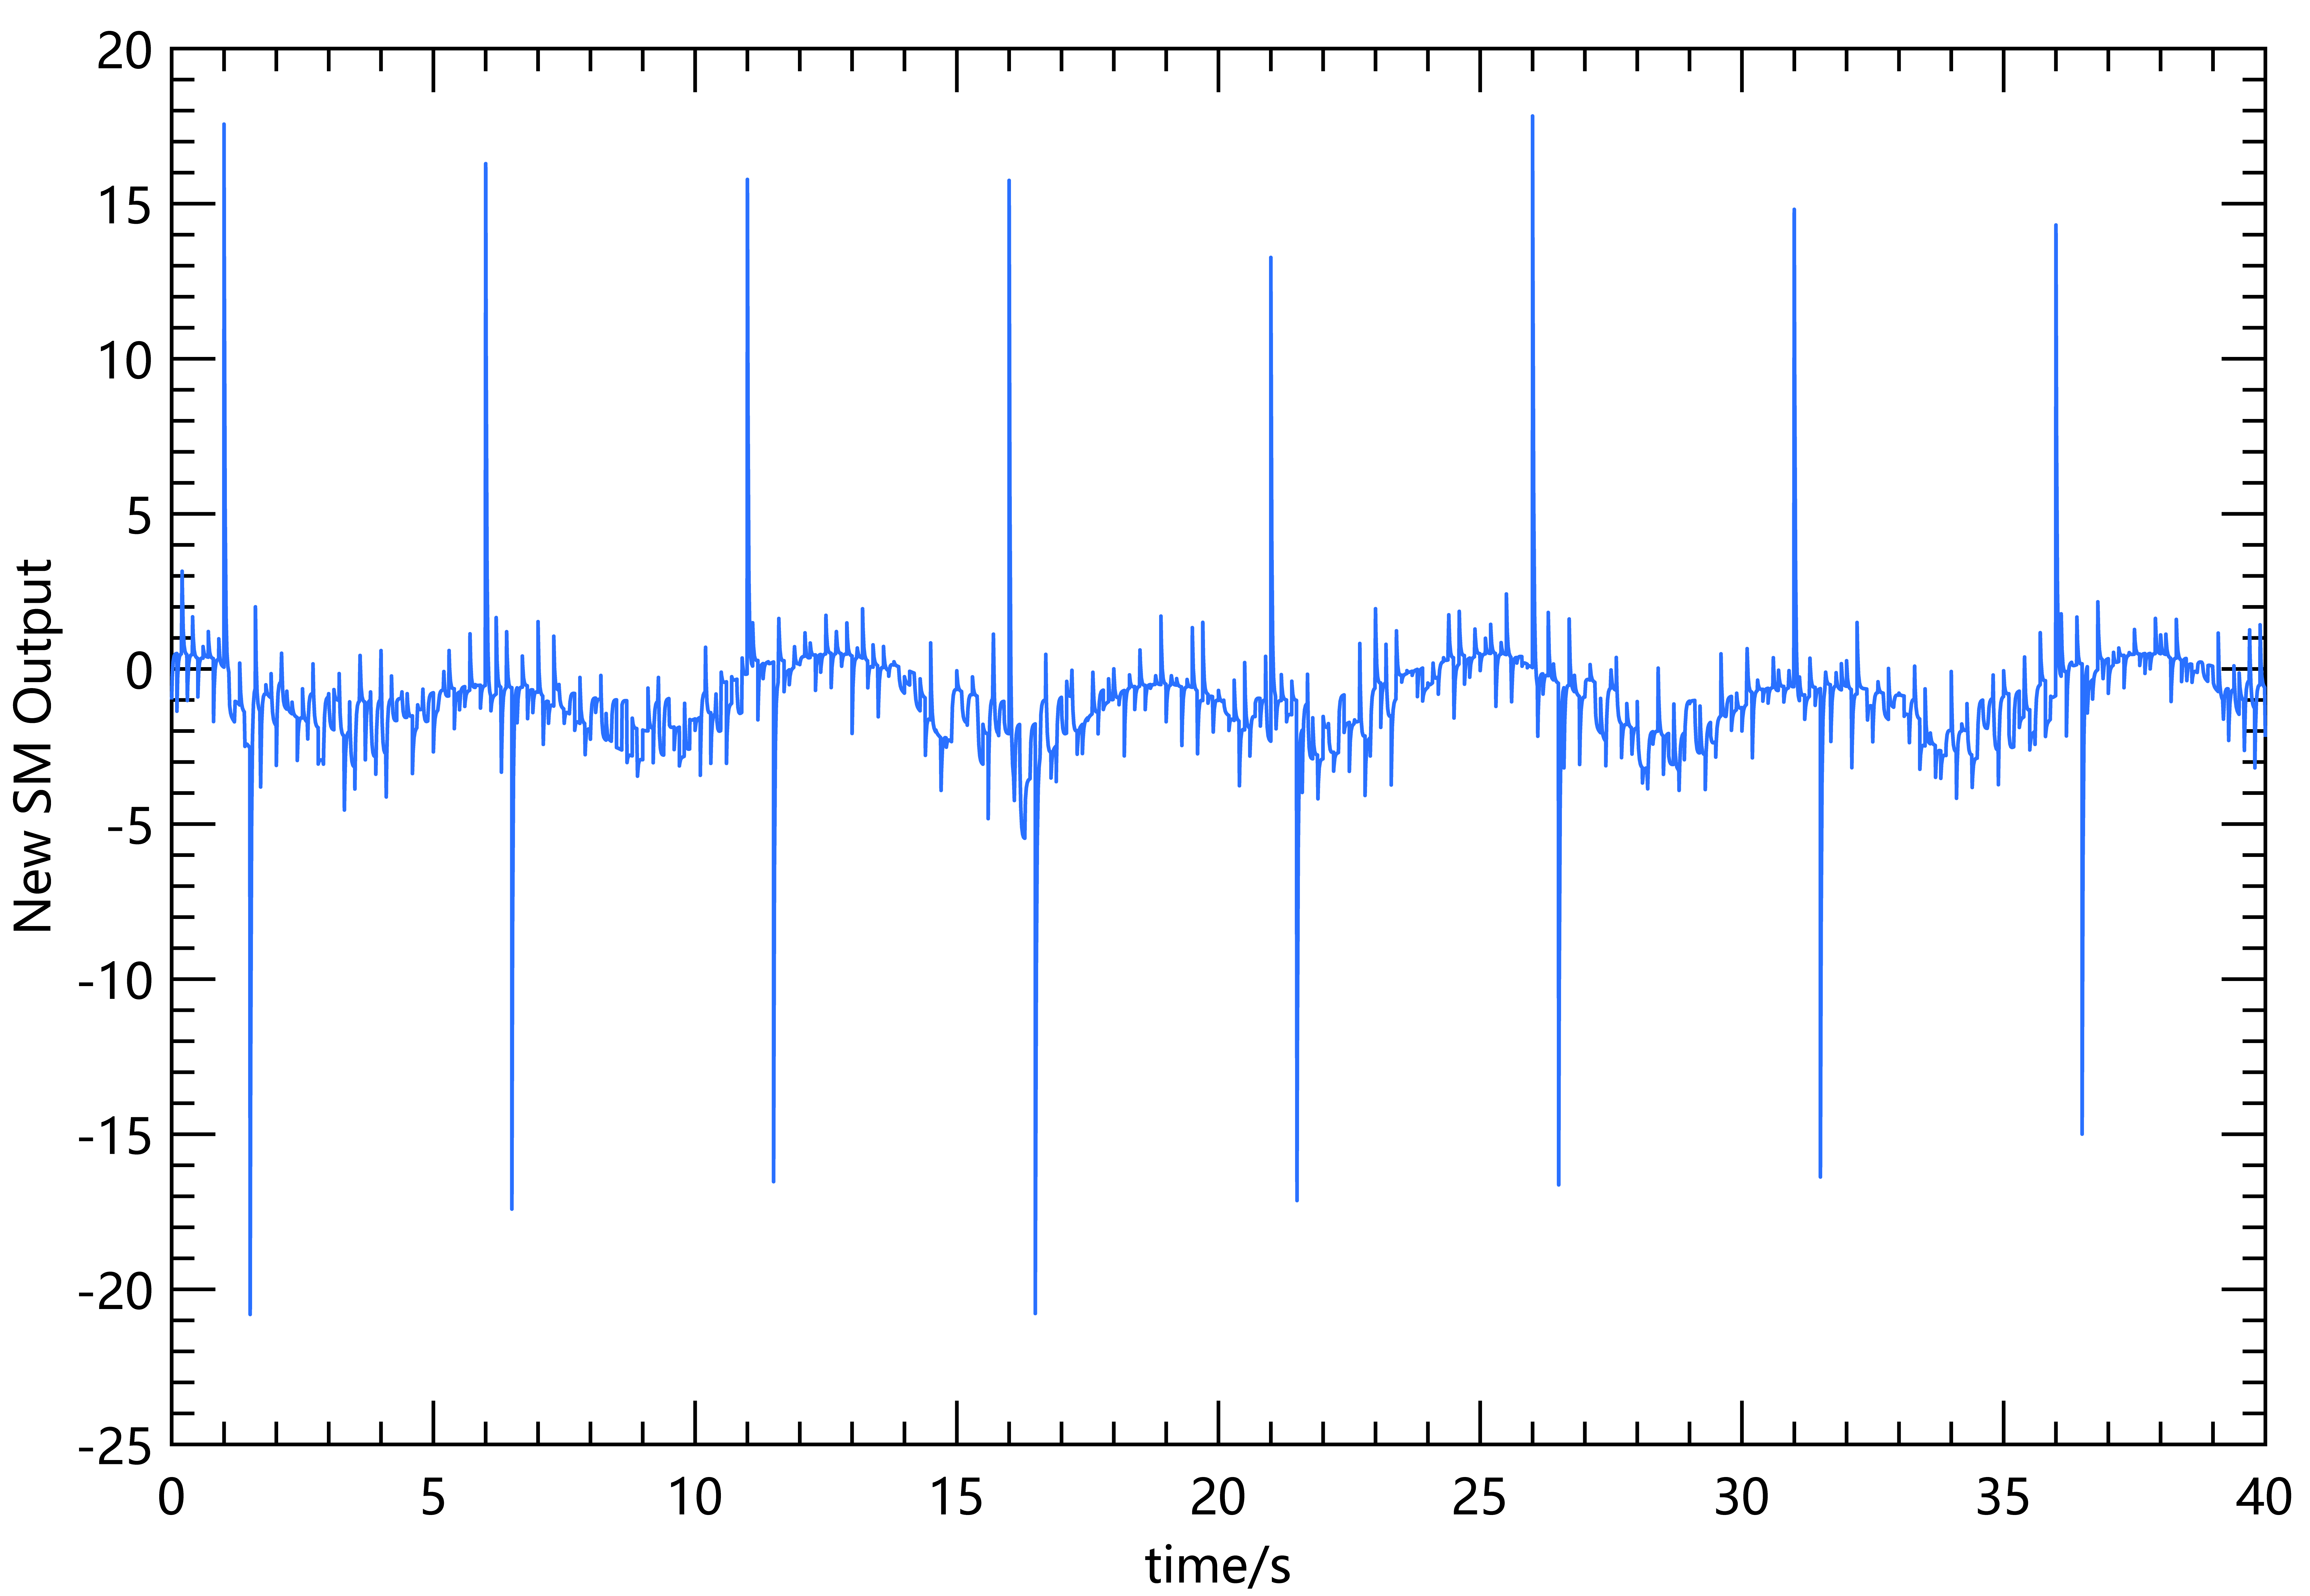
\includegraphics[width=0.9\textwidth]{imgs/simu_pulse_sine_u1.png}
    % \caption{}
    \end{minipage}%
    }%
    \centering
    \caption[]{控制器输出对比}
    \label{fig:simu_pulse_sine_u}
\end{figure}

可以发现,两个控制器对外界扰动响应都很灵敏,自适应控制器对误差的响应更快、准确,但其仍然存在抖动频率太高这一缺点,而这在本文提出的控制器中是不存在的。与此同时,本文的控制器在遭遇扰动时会输出一个相对高的值,其余时刻,尽管存在观测扰动误差,其输出值仍然较小,输出频率也可以忍受。

总的来说,本文提出的控制器有下面几个特点:

\begin{enumerate}
    \item 控制器理论上稳定,收敛速度快
    \item 控制器不需要具体动力学模型,参数易调节
    \item 对扰动误差鲁棒性好
    \item 控制器输出相对光滑,频率低,可以直接应用在机械装置上
\end{enumerate}

但在前面的仿真实验中也可以发现,在遭遇大的扰动时,控制器会输出一个相对高的值(尽管相对普通滑膜控制器较小),这可能会影响实际机构的运行。因此,为了解决这一问题,采用简单的凸优化规划器,通过控制期望步长之间的速度、加速度,将大的扰动分散到几步来实现,保证控制器对扰动的响应更加平滑。
\FloatBarrier
\subsection{凸优化规划器}

我们考虑使用凸优化的方法为运动控制添加约束,保证给定的控制曲线尽量平滑连续。

对单根轴而言,为了增强对突然大扰动的抵抗力,设定轴的运动曲线满足一定的速度约束和加速度约束。为了简单起见,将问题约定如下:

记轴的长度为$l_i$,$i$代表时刻$t_i$下的轴长。控制给定当前时刻$t_k$和前一时刻$t_{k-1}$的轴长$l_{k}$、$l_{k-1}$。我们期望在之后时刻$t_{k+N}$有$l_{k+N}=l_{k}^*$,其中$l_{k}^*$代表$t_k$时刻给定的期望目标。因此问题整理为下面的优化问题(\ref{eqn:convex_problem}):

\begin{equation}
    \begin{aligned}
        \min &\left| l_{k}^{*}-l_{k+N} \right|^2+\lambda \sum_{i=1}^N{\left( l_{k+i}-l_{k+i-1} \right) ^2}\\
        \mathrm{s}.\mathrm{t}.\quad &\begin{array}{c}
        \left| \frac{l_{k+i+1}-l_{k+i}}{t_s} \right|\le v_{\max}, \quad i=0,1,\cdots ,N-1\\
        \left| \frac{l_{k+i+1}+l_{k+i-1}-2l_{k+i}}{{t_s}^2} \right|\le a_{\max}, \quad i=0,1,\cdots ,N-1\\
    \end{array}\\
    \end{aligned}
    \label{eqn:convex_problem}
\end{equation}

将问题整理成矩阵形式。

记需要规划的向量为式子(\ref{eqn:convex_x})
\begin{equation}
    {x}=\left( \begin{array}{c}
        l_{k+1}\\
        l_{k+2}\\
        \vdots\\
        l_{k+N}\\
    \end{array} \right) 
    \label{eqn:convex_x}
\end{equation}

由于问题是一个二次方程形式,可以整理优化函数为二次凸优化形式(\ref{eqn:convex_target})。

\begin{equation}
    \begin{aligned}
        F&=\min \left| l_{k}^{*}-l_{k+N} \right|^2+\lambda \sum_{i=1}^N{\left( l_{k+i}-l_{k+i-1} \right) ^2}\\
        &=\frac{1}{2}x^THx+f^Tx\\
    \end{aligned}
    \label{eqn:convex_target}
\end{equation}

其中有(\ref{eqn:convex_H}):

\begin{equation}
    \begin{array}{c}
        H=\hat{H}+\hat{H}^T\\
        \hat{H}=\left( \begin{matrix}
        2\lambda&		&		&		\\
        -2\lambda&		\ddots&		&		\\
        &		\ddots&		2\lambda&		\\
        &		&		-2\lambda&		1+\lambda\\
    \end{matrix} \right) \quad f=\left( \begin{array}{c}
        -2\lambda l_k\\
        0\\
        \vdots\\
        0\\
        -2l^*\\
    \end{array} \right)\\
    \end{array}
    \label{eqn:convex_H}
\end{equation}

对于约束,可以将其表示为式子(\ref{eqn:convex_Av}-\ref{eqn:convex_b}):

\begin{equation}
    A_v=\left( \begin{matrix}
        1&		&		&		\\
        -1&		1&		&		\\
        &		-1&		\ddots&		\\
        &		&		-1&		1\\
    \end{matrix} \right) _{N\times N}\quad A_a=\left( \begin{matrix}
        1&		&		&		&		\\
        -2&		1&		&		&		\\
        1&		-2&		1&		&		\\
        &		\ddots&		\ddots&		\ddots&		\\
        &		&		1&		-2&		1\\
    \end{matrix} \right) _{N\times N}
    \label{eqn:convex_Av}
\end{equation}

\begin{equation}
    A=\left( \begin{array}{c}
        A_v\\
        -A_v\\
        A_a\\
        -A_a\\
    \end{array} \right) _{4N\times N}
\end{equation}

\begin{equation}
    b_v=t_sv_{\max}\left( \begin{array}{c}
        1\\
        1\\
        \vdots\\
        1\\
    \end{array} \right) _{2N\times 1}+\left( \begin{array}{c}
        l_k\\
        0\\
        \vdots\\
        0\\
    \end{array} \right) _{2N\times 1}\quad 
\end{equation}

\begin{equation}
    b_a={t_s}^2a_{\max}\left( \begin{array}{c}
        1\\
        1\\
        \vdots\\
        1\\
    \end{array} \right) _{2N\times 1}+\left( \begin{array}{c}
        0\\
        \vdots\\
        0\\
        \underset{row\,\,N+1}{\underbrace{2l_k-l_{k-1}}}\\
        \underset{row\,\,N+2}{\underbrace{-l_k}}\\
        0\\
        \vdots\\
        0\\
    \end{array} \right) _{2N\times 1}
\end{equation}

\begin{equation}
    b=\left( \begin{array}{c}
        b_v\\
        b_a\\
    \end{array} \right) _{4N\times 1}
    \label{eqn:convex_b}
\end{equation}

满足式子(\ref{eqn:convex_Ax}):
\begin{equation}
    {Ax}\le {b}
    \label{eqn:convex_Ax}
\end{equation}
因此,整体问题可以表示为带约束的二次凸优化情形,具体形式为式子(\ref{eqn:convex_result}):

\begin{equation}
    \begin{array}{c}
        \min  F=\frac{1}{2}x^THx+f^Tx\\
        \mathrm{s}.\mathrm{t}.\quad Ax\le b\\
    \end{array}
    \label{eqn:convex_result}
\end{equation}

这类问题具有很多成熟的解,本文选用内点法完成求解。

\FloatBarrier
